\documentclass{Class/class}
\usepackage[utf8]{inputenc}
\usepackage[T1]{fontenc} 
\usepackage{subcaption}

\usepackage{color}
\usepackage{lipsum}
\usepackage{array}
\usepackage{amsmath}
\usepackage{float}
\usepackage{listings}     % Package for including code snippets
\usepackage{xcolor}       % For custom colors
\usepackage{tikz}
\usepackage{graphicx}


% Define a new language for your programming language
\lstdefinelanguage{Bleach}{
    % Define keywords
    morekeywords={and, break, class, continue, do, elif, else, false, for, function, if, inherits, lambda, let, method, nil, or, print, return, self, super, true, while},
    % Define other keywords (e.g., types or built-ins) with different styles
    morekeywords=[2]{std::chrono::clock, std::io::readLine, std::io::print, std::io::fileRead, std::io::fileWrite,
    std::math::abs, std::math::fmod, std::math::log, std::math::pow", std::math::sqrt, std::random::random,
    std::utils::ord, std::utils::numToStr, std::utils::strToNum, std::utils::strToBool, std::utils::strToNil},
    % Define comments
    comment=[l]{//}, % Line comment with //
    morecomment=[s]{/*}{*/}, % Block comment between /* and */
    % Define string delimiters
    morestring=[b]", % Strings are enclosed in double quotes
    % Styling for different parts
    keywordstyle=\color{blue}\bfseries,   % Style for keywords (bold blue)
    keywordstyle=[2]\color{teal},         % Style for secondary keywords (teal)
    commentstyle=\color{gray}\itshape,    % Style for comments (italic gray)
    stringstyle=\color{red},              % Style for strings (red)
    numberstyle=\tiny\color{gray},        % Line numbers style (tiny gray)
    backgroundcolor=\color{white},        % Background color (optional)
    showstringspaces=false,               % Don't show spaces in strings
}

\lstset{
    language=Bleach, % Change to your language
    basicstyle=\ttfamily\small,
    keywordstyle=\color{blue},
    commentstyle=\color{gray},
    stringstyle=\color{red},
    numberstyle=\tiny\color{gray},
    numbers=left,
    stepnumber=1,
    breaklines=true,
    frame=single,
}

\newcommand{\Fix}[1]{[\textbf{TODO}: {\color{red} #1}]}
\newcommand{\atencao}[1]{[\textbf{!!ATTENTION!!}~{\color{red} #1}]}
\newcommand{\lmt}[1]{[\textbf{Leopoldo}:~{\color{orange} #1}]}


\usepackage[linesnumbered,ruled,vlined]{algorithm2e}
\usepackage{csquotes}
\begin{document}
\newcommand{\numprotocolos}[1][16]{#1 }

\frontmatter

\newpage
\begin{titlepage}
    \thispagestyle{empty}
    \begin{center}
    
\includegraphics[width=3cm]{Figures/logoufpe.jpg}
  \large
  \\Universidade Federal de Pernambuco
  \\Centro de Informática
  \vskip 25mm
  Bachelor's Degree in Computer Engineering
  \vskip 45mm
  \begin{minipage}{160mm}
    \begin{center}
      \textbf{Bleach: A programming language aimed for teaching introductory "Compilers" courses.}
      \vskip\baselineskip
      Victor Miguel de Morais Costa
      \vskip\baselineskip
      Undergraduate Thesis
    \end{center}
  \end{minipage}\\
  \vfill
  Recife, Pernambuco\\
  October , 2024
  \end{center}
\end{titlepage}
\newpage
\thispagestyle{empty}
    \begin{center}
    \large
    Universidade Federal de Pernambuco\\
    Centro de Informática\\
    \vskip 25mm
    Victor Miguel de Morais Costa
    \vskip\baselineskip
    \textbf{Bleach: A programming language aimed for teaching Compilers}
  \vskip 58mm
  \begin{flushright}
    \begin{minipage}{100mm}
    \small{
    Work presented to the Undergraduate Course in Computer Engineering at the Informatics Center of the Federal University of Pernambuco as a partial requirement to obtain the Bachelor's degree in Computer Engineering.}
    \vskip2\baselineskip
    \small{\textbf{Concetration Area: Programming Languages} }
    \newline \small{\textbf{Advisor: Leopoldo Teixeira} }
    %\newline \small{\textbf{Co-orientador:} }
    \end{minipage}
  \end{flushright}
  \vfill
  Recife, Pernambuco\\
  October, 2024
  \end{center}
\newpage
  \thispagestyle{empty}
  ~\\
  \vfill
  \begin{flushright}
    \begin{minipage}{80mm}
    \textit{Dedico este trabalho a Deus e minha família.}
    \end{minipage}
  \end{flushright}
\thispagestyle{empty}
\begin{spacing}{1.0}
\chapter*{Acknowledgments}

Andrea,

Alvaro,

Maria Dolores,

Laura,

Leopoldo Motta Teixeira,

Fernando Castor, Gustavo Carvalho,

Daniel Perazzo, Fernando Macedo, Lucas Ambrosio, Matheus Teotônio, Riei Joaquim, Victor Hugo, Victor Ximenes, Zênio Ângelo

José Carlos da Silva Cruz, Pedro Nogueira Coutinho, Zilde Souto Maior Neto

José Victor Silva Cruz, Lucas Santana, Marcos Oliveira,

Cintia,

Noriaki Kubo,
    
\clearpage
\end{spacing}
\newpage
\thispagestyle{empty}
  ~\\\vfill
\begin{flushright}
    \begin{minipage}{0.6\textwidth}
      \begin{flushright}
        \begin{quote}
           \textit{``The ocean is full 'cause everyone's crying \newline
           The full moon is looking for friends at high tide \newline
           The sorrow grows bigger when the sorrow's denied \newline
           I only know my mind \newline
           I am mine \newline
           \newline
           And the meaning, it gets left behind \newline
           All the innocence lost at one time \newline
           Significant, behind the eyes \newline
           There's no need to hide \newline
           We're safe tonight \newline
           \newline
           And the feelings that get left behind \newline
           All the innocence broken with lies \newline
           Significance, between the lines \newline
           We may need to hide \newline
           \newline
           And the meanings that get left behind \newline
           All the innocence lost at one time \newline
           We're all different behind the eyes \newline
           There's no need to hide, yeah"} 
        \end{quote}
        \vskip.2\baselineskip%
        --- "I am Mine", Pearl Jam, 2002
      \end{flushright}
    \end{minipage}
\end{flushright}


%\maketitle

\thispagestyle{empty}
\begin{spacing}{1.0}
\chapter*{Resumo}
Nos cursos de bacharelado em Ciência da Computação ou Engenharia da Computação, espera-se que os alunos tenham contato com uma disciplina de Compiladores de nível introdutório. Devido à grande amplitude e complexidade dos temas abordados nesta disciplina, os professores responsáveis tendem a conduzi-lá sob um ponto de vista mais teórico. 

Esta abordagem costuma proporcionar aos alunos uma compreensão mais profunda dos conceitos fundamentais desta área e prepará-los melhor para uma carreira orientada para a pesquisa científica. No entanto, tende a limitar a experiência prática dos conceitos ensinados, fazendo com que os alunos muitas vezes se sintam desconectados das aplicações dessa área, causando um menor engajamento e motivação entre estes. Diante disso, desde a década de 90, novas metodologias, que mesclam teoria e prática, começaram a surgir. Na maioria delas, os alunos devem implementar um compilador ou um interpretador para uma linguagem de programação de fins didáticos, normalmente definida pelo professor responsável.

Devido às desvantagens mencionadas da abordagem tradicional e às limitações que algumas das linguagens propostas na abordagem mista apresentam, a proposta atual visa apresentar uma nova linguagem de programação chamada Bleach, juntamente com uma implementação de seu interpretador. Tal linguagem pretende ser utilizada como ferramenta em disciplinas introdutórias de Compiladores que optem por seguir uma abordagem de ensino mais voltada para a prática incremental, priorizando a flexibilidade e objetivando solucionar, ou pelo menos mitigar, as desvantagens de ambas as abordagens mencionadas. No entanto, é essencial esclarecer que a avaliação de Bleach no contexto educacional não faz parte do escopo do trabalho aqui apresentado.

\textbf{Palavras-chave:} Compiladores; C++; Educação; Software Educacional; Interpretadores; Linguagens de Programação.
        
\clearpage
\end{spacing}
\chapter*{Abstract}
\begin{spacing}{1.0}
In Bachelor's degrees in Computer science or Computer engineering, students are expected to have contact with an introductory-level Compilers course. Due to the large breadth and depth of topics in this subject, professors and instructors tend to conduct it from a more theoretical point of view. 

This approach tends to provide students a deeper understanding of the fundamental concepts of this field and better prepare them better for a research oriented career. However, it tends to limit the hands-on experience of the taught concepts, making students often feel disconnected from real-world applications of this area, causing less engagement, excitement and motivation among them. Given this, since the 90s, new methodologies, which combined theory and practice, began to emerge. In most of them, students we required implement a compiler or an interpreter for a programming language for teaching purposes, normally defined by the responsible professor or instructor.

Due to the aforementioned disadvantages of the traditional approach and the limitations that some of the proposed programming languages in the mixed approach present, this proposal aims to present a new programming language called Bleach along with an implementation of its interpreter. This language is intended to be used as a tool in introductory-level Compilers courses whose responsible professors opt to follow a teaching approach more focused on incremental practice, prioritizing flexibility and aiming to solve, or at least mitigate, the disadvantages of both mentioned approaches. However, it is important to highlight that the assessment of Bleach in the educational context is out of the scope of the thesis presented here.



\textbf{Keywords:} Compilers; C++; Education; Educational Software; Interpreters; Programming Languages.  

\end{spacing}
\listoftables
\listoffigures
\tableofcontents

\mainmatter

\chapter{Introduction} \label{cap:introduction}

\begin{displayquote}
    \begin{center}
        \textit{``If you were to give me wings, I would fly for you. Even if this entire land were to sink underwater. If you were to give me a sword, I would stand up and fight for you. Even if the entire sky were to pierce you with its light.''}
    \end{center}
\end{displayquote}

\begin{flushright}
   \textit{-- NORIAKI KUBO}
\end{flushright}

\section{Background and Motivation}
In Computer Engineering and Computer Science programs, the Compilers course is essential for development of students' knowledge in this area, since it provides the basis of how programming languages are executed by computers.

As stated in \cite{aho2008teaching}, in Compilers courses, practical experience is a very important aspect since it allows the students exercise the learned theoretical concepts in the classes. Due to this scenario, efforts have been made since this topic started being taught at universities, in order to build learning tools focused on theoretical aspects. However, in certain cases there is still a lack of practical tool that are capable of allowing students to get their hands dirty and work with compiler components.

Given this context, it becomes clear that there exists a gap when it comes down to learning tools focused in practical aspects. Therefore, the opportunity to design and implement a specialized programming language to address these educational challenges emerged.

\section{The Problem}
When analyzing the structure of initial and traditional Compilers courses, it is noticeable that they often rely too much on theoretical lectures and, in some cases, on code examples that fail to engage and motivate undergraduate students that are having their first contact with compilers design and implementation.

Given this past scenario, changes started to being made in order to offer a better and more fruitful learning experience through the creation of different educational programming languages. Unfortunately, even though the intentions were good, when analyzing them in retrospect, it is safe to conclude that most of them are either too simple and uninteresting to demonstrate real-world compiler concepts or too complex and overwhelming for students to work with in an educational setting that usually spans across just one academic semester.

By examining these circumstances and the history behind programming languages and compilers development, it became clear that currently there is a lack of programming languages that could effectively used in balancing educational clarity and practical experimentation. Having this obstacle in mind, this thesis seeks to offer a new solution for this problem, by focusing more on teaching just the essential concepts and giving the students the chance to practice as much as they can, instead of spending too much time on theoretical aspects of this field.

\section{Objectives}
The main goal of this undergraduate thesis is to present a programming language specifically designed and implemented for use in undergraduate Compilers courses at Computer Engineering and Computer Science programs.

The language aims to offer a practice-oriented understanding of core compiler and interpreter phases such as lexical analysis, syntax parsing, semantic resolution, and interpretation.

Finally, by allowing the students to implement and interact with these components in an active learning environment, Bleach seeks to create a better connection between theoretical knowledge and practical application.

\section{Scope}
It is very important to highlight to the reader that this undergraduates thesis' focus is exclusively on the presentation, implementation and evaluation of a programming language that was designed to simplify the understanding of compiler phases, particularly lexical analysis, syntax analysis, semantic resolution and interpretation. In other words, this thesis aims to defend a new point of view where teaching interpreters implementation instead of compilers is a reasonable and valuable approach that is supposed to not overwhelm students who are having their first contact with the subject. Moreover, as previously mentioned, the assessment of Bleach in the educational context is out of the scope of the work presented here.

Therefore, the implementation of the programming language presented here will not address advanced compiler topics, such as: type systems, code optimization, register allocation, or machine code generation, since each one of them is complex enough to be studied by several weeks.

Instead, the language implementation presented here will emphasize core concepts in an accessible way to undergraduate students.

\section{Contributions}
The main contribution of this thesis is the design and implementation of a new programming language specifically tailored for teaching Compilers courses.

The language’s simplicity allows students to experiment with real compiler phases without being overwhelmed by the complexities of full-scale language implementations.

On top of that, the language provides detailed feedback at each stage of the interpreting pipeline, helping students to have a more solid comprehension of this area. Also, the implementation of the language has its own test suite, that can, and should be, used by the teaching staff during the course.

\section{Thesis Structure}
Ultimately, this thesis is structured in the following format: Chapter 2 provides a literature review that discusses essentials theoretical concepts of the programming language design and implementation field. Chapter 3 is dedicated to provide a historical context about how the teaching of this subject evolved during the last 60 years and also to show studies that highlight the importance of a practice-oriented approach in Compilers courses. This chapter also provides an overview of existing programming languages that attempt to solve the same problem exposed in this chapter. Then, Chapter 4 presents Bleach, the programming language proposed as a new solution for the mentioned issue. The chapter goes deep into the features that the language has and gives a brief overview of its standard library. After this, an in-depth analysis of how each component of the implemented interpreter is presented and, it ends with a discussion about the challenges when designing and implementing the language, as well as the trade-offs made during these two processes. Chapter 5 goes into the evaluation aspect of the language, by explaining how its test suite works. Then, as a statement of it expressiveness, a link to a GitHub repository containing implementations of famous algorithms and data structures is presented to the reader. Concluding the chapter, a brief feature comparison between Bleach and its competitors is shown, proving that Bleach is, indeed, a viable option to choose when teaching Compilers courses. At last, Chapter 6 concludes this thesis by reflecting on the contributions that were made and opportunities of future work and enhancements regarding Bleach.
\chapter{Theoretical Review} \label{Cap:theoretical_review}

\begin{displayquote}
    \begin{center}
        \textit{``Do not live bowing down. Die standing up.''}
    \end{center}
\end{displayquote}

\begin{flushright}
   \textit{-- NORIAKI KUBO}
\end{flushright}

% \section{Introduction}
This chapter is dedicated to provide a literature review about the Programming Language Design and Compiler/Interpreter Implementation fields. The conceptual content presented here is heavily influenced by \cite{aho1986compilers}, \cite{cooper2022engineering} and \cite{nystrom2021crafting}.

\section{What is a Compiler and How does it work?}
To simply put it simple, a compiler is a software whose responsibility is to translate a program written in a certain programming language into a another program written in another one, without modifying the meaning of the original program, that is, its semantics. However, despite this simple description, compilers are usually complex and large software systems composed of several components which interact with each other during the mentioned translation process, commonly known as compiling.

The importance of compilers in both computer science and real-world applications is immeasurable. The key points below illustrate some of the most prominent impacts of this creation:

\begin{itemize}
    \item \textbf{Bridging High-Level Languages to Machine Code:} As previously mentioned, the purpose of a compiler is the translation between programs written in different programming languages. Usually, in practice, such translation happens from a high-level programming language, commonly more human-readable and that provides several abstractions, into a programming language that is closer to the hardware and, therefore, more machine-readable. Given this fact, it is safe to say that a compiler provides several layers of abstractions that allow developers to build complex software that impact people's life around the world since its conception.
    
    \item \textbf{Impact on Portability:} One of the major features of compilers is their portability. In practice, this means that code once a program, written in a high-level programming language, passes through the compiling process, the resulting machine-code can be used in different hardware platforms by simply targeting different machine architectures, such as: x86, ARM, RISC-V, MIPS and others. This allows the same code base to be re-used in independent systems without the need to rewrite the code base in order to target each different architecture.
    
    \item \textbf{Programming Languages Evolution:} In the current context, it is crucial to reiterate that compilers and programming languages are deeply tied. In practice, the evolution of one serves as a trigger to the evolution of the other and vice-versa. Compilers permit language designers to experiment on new ideas that cross different programming paradigms, such as the procedural, object-oriented, functional, aspect-oriented, concurrent and several others. Furthermore, the evolution of existing programming languages and creation of new ones may allow the enhancement of existing compilers and creation of new ones for niche areas.
    
    \item \textbf{Impact on Software Development:} Without the existence of compilers, the development of software applications would become far more difficult since there would be no bridge uniting codebases written in high-level languages and hardware systems where such codebases are executed. Therefore, this would limit the growth of technology-based companies.
\end{itemize}

Given the impacts emerged from the creation of compilers, now it is time to take a deep dive into how this particular type of software works.

As already explained, a compiler is a complex software system and due to this, must be structurally organized in components responsible for executing a single task in the compiling procedure. According to \cite{cooper2022engineering}, compilers are being implemented since 1955. During these early years of development, a compiler was viewed as a tool that had to understand the program written in the source language and translate it, without altering its meaning, to a target architecture. The distinction between these two tasks, made computer scientist adopt the following structuring when it came down to the components of a compiler: each compiler should have a front-end and a back-end. 

In conformity with what has been exposed, the front-end was responsible for understanding the program written in the source language, while the back-end's responsibility lied on the process of mapping programs to machines. As the reader might have already thought, there must be some kind of link between the front-end and the back-end. That is where the Intermediate Representation (IR) comes in. The front-end must encode the needed information about the source program in some way, so it can be properly used by the back-end when it starts the mentioned mapping process later on. The Intermediate Representation is the entity that contains such information generated by the front-end. It is considered the definitive representation of the source code that will be transformed into machine-code by the back-end.

In short, it can be said that the front-end's responsibility is guarantee that the source code is well-formed and also translate it to the intermediate representation. On the other side, the back-end's duty is translate such intermediate representation into the machine-code of a specific machine architecture, respecting the physical limitations of the target hardware.

As the decades passed on, the process of designing and implementing a compiler became more sophisticated as the structure of such system became increasingly more complex and robust.

\newpage

Shifting the focus of compilers' implementation to a classroom environment, it is safe to expect that students are capable of implementing more sophisticated compilers that have the following structure, which is not that far from those used in the industry:

\begin{figure}[H]  
  \centering
  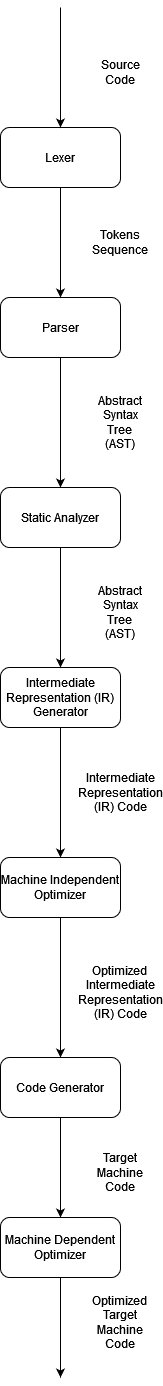
\includegraphics[width=\textwidth, height=0.8\textheight, keepaspectratio]{Figures/Arquiteturas/CompilersDetailedPipeline.png}  
  \caption{A detailed compiler structure}
  \label{fig:comp}
\end{figure}

\newpage

It is also completely plausible to simplify this task by asking the students to implement a compiler that follows the following simplified structure:

\begin{figure}[H]  
  \centering
  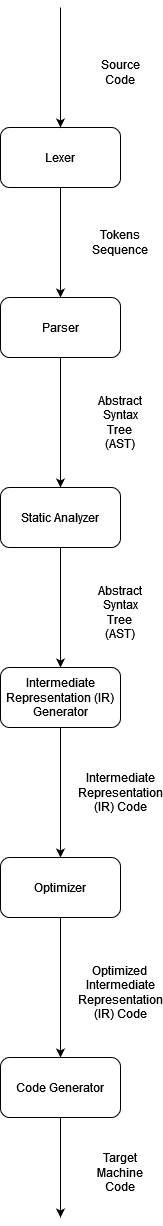
\includegraphics[width=\textwidth, height=0.8\textheight, keepaspectratio]{Figures/Arquiteturas/CompilersSimpliefiedPipeline.png}  
  \caption{A simplified compiler structure}
  \label{fig:Fluxograma}
\end{figure}
    
Section 2.4 is dedicated to provide an in-depth overview of each of the compiler's components from the simplified structure presented in the image above.


\section{What is an Interpreter and How Does it Distinguishes Itself From a Compiler?}
In order to explain what is an interpreter, it is necessary to recall the reader what is a compiler and what constitutes the compiling process.

A compiler is a program that takes as input a specific programming language and translates it to another, but without executing it. This step is delegated to the users, who must execute it by themselves.

In essence, compiling means translating code written in a source programming language to a target programming language (that is usually in a lower level, when compared to the source one). Whether the compiler generates machine code or bytecode, it is still performing a compiling process.

Once the reader has remembered what a compiler does and what compiling is, an interpreter is a program that takes as input a specific programming language and immediately executes it.

Keith Cooper and Linda Torczon provide another point of view to the discussion about the distinctions between compilers and interpreters in \cite{cooper2022engineering}.

According to them, a compiler is a type of software responsible for taking as input a program written in a certain source programming language and producing as output a representation of this very same program as a sequence of the instructions available at the target machine. Normally, the source programming language can be C, C++, Fortran, Java, and ML, while the "target" programming language is just the instruction set of a specific computer architecture (ARM, RISC-V, MIPS, x86, etc).

An interpreter, in contrast, receives as input a program written in a certain programming language, but its output is the result of executing the code written in the source language. Some language that fall into this category are: Perl and Scheme.

The images shown below are good examples that illustrate the input and the output of both compilers and interpreters:

\begin{figure}[H]  
  \centering
  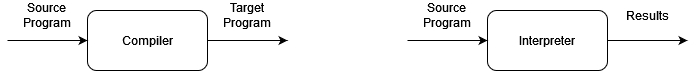
\includegraphics[width=\textwidth, height=\textheight, keepaspectratio]{Figures/Arquiteturas/Compilers and Interpreters.png}  
  \caption{Compilers and Interpreters}
  \label{fig:CompilersAndInterpreters}
\end{figure}

Finally, it is also highlight that there are some programming languages, such as Java and Python, whose implementations combine both compiling and interpreting. Considering Java as example, its implementation compiles the program written in the language to a bytecode format. Then, once the program is in the bytecode format, the Java Virtual Machine (JVM) executes the Java application (bytecode format) by running this bytecode inside the JVM (which can also be viewed as an interpreter for this lower-level representation). A similar process is followed by the Python programming language.

With this, it is reasonable to conclude that compilers and interpreters have a lot in common, due to the fact that they perform almost the same set of tasks, such as:
\begin{itemize}
    \item Analysis of the input program written in the source language in order to figure out if it is a valid one or not.
    \item Construction of internal models that are used to better understand the structure and meaning (semantics) of the input program.
    \item Determination of where to store values during the execution of the input program.
    
\end{itemize}

\section{Detailed Overview of Compiler's Components}

\subsection{Lexer}
The lexer is the first component present in the compiling process of a compiler. It is responsible for executing a process called lexing, which is also known as lexical analysis.

As earlier elucidated, the input of a compiler is the source code of a program written in a specific programming language. The content present inside the source code is viewed by the compiler as a large string, a linear sequence of characters, that has no meaning for it at all at this stage. The lexer's goal is to transform this sequence of characters that is the source code into a new representation that is more abstract from the compiler's perspective, so it can be passed on to the next component, the parser.

To perform such procedure, the lexer takes in this stream of characters and group them together forming a sequence of entities that convey the idea of a "word". These entities are called tokens.

Making an analogy to linguistics, one can say that the lexer's purpose is to group letters (characters) into words (tokens). Given this analogy, it is essential to inform the reader that, like words, tokens can have different lengths and different meanings. Some examples are listed below to better illustrate a few cases:
\begin{itemize}
    \item Single-Character Tokens: \texttt{(}, \texttt{\{}, \texttt{+}, \texttt{-}, \texttt{*}, \texttt{/}, etc.
    \item Double-Character Tokens: \texttt{==}, \texttt{!=}, \texttt{>=}, \texttt{<=}, etc.
    \item Multi-Character Tokens: \texttt{123} (a number literal), \texttt{"hello"} (a string literal), \texttt{true} (a boolean literal), \texttt{aVariable} (an identifier), etc.
\end{itemize}

It is also important to mention that certain characters have no meaning for the lexer during the lexical analysis and, therefore, are completely ignore in the process, such as: whitespace characters and characters that represent comments in the programming language in which the source file was written.

By the end of the lexical analysis, the sequence of characters is transformed into a sequence of tokens by following the syntax rules of the source programming language.

The figure below shows, in an simple example, the input and the output of this component:

\begin{table}[H]
    \centering
    \begin{tabular}{|c|c|c|c|c|c|c|c|c|c|c|c|c|c|c|c|c|c|c|c|c|}
        \hline
        l & e & t &  & a & v & g &  & = & ( & m & i & n & + & m & a & x & ) & / & 2 & ; \\
        \hline
    \end{tabular}
\end{table}

\begin{figure}[H]
  \centering
  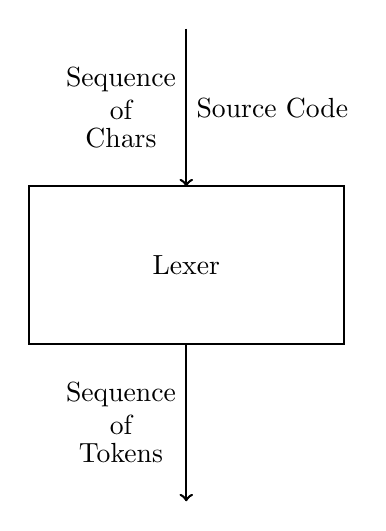
\begin{tikzpicture}
    % Draw the boxes
    \draw[thick] (0, 0) rectangle (4, 2);
    
    % Labels inside the boxes
    \node at (2, 1) {Lexer};

    % Input and output arrows
    \draw[->, thick] (2, 4) -- (2, 2) node[midway, left] {\shortstack{Sequence\\ of\\ Chars}};
    \draw[->, thick] (2, 4) -- (2, 2) node[midway, right] {\shortstack{Source Code}};
    \draw[->, thick] (2, 0) -- (2, -2) node[midway, left] {\shortstack{Sequence\\ of\\ Tokens}};
    \draw[->, thick] (2, 0) -- (2, -2) node[midway, left] {\shortstack{ }};
  \end{tikzpicture}
\end{figure}

\begin{table}[H]
    \centering
    \begin{tabular}{|c|c|c|c|c|c|c|c|c|c|c|}
        \hline
        let & avg & = & ( & min & + & max & ) & / & 2 & ; \\
        \hline
    \end{tabular}
\end{table}

\begin{figure}[H]  
  \caption{Input and Output of a Lexer}
  \label{fig:lexer}
\end{figure}

As seen in the example above, the lexer receives a sequence of characters, which represents the raw source code, and gives as the result a series of chunks of characters called tokens. Making another analogy with linguistics, one can think of tokens as the "words" and  the "punctuation" that constitutes a programming language.

Going further, it is also possible to say that the lexer's job is execute a traversal through the sequence of characters received and group such characters into the smallest sequences that represent something in the source programming language. Each of these resulting sequences of grouped characters is called a lexeme.

Therefore, in the example presented above, the sequence of lexemes produced from analyzing the sequence of characters received as input was: \texttt{let}, \texttt{avg}, \texttt{=}, \texttt{(}, \texttt{min}, \texttt{+}, \texttt{max}, \texttt{)}, \texttt{/}, \texttt{2}, \texttt{;}

In conclusion, lexemes are just raw substrings presented in the source code.

However, a token is much more than a lexeme. It generally contains other pieces of information that are useful in further stages of the compiling process and also in error report.

Usually, each token has a token type associated. For example, the lexeme \texttt{2} usually has \texttt{NUMBER} as its token type, while \texttt{+} often has \texttt{PLUS} as its token type. In this context, it is relevant to highlight that the amount of token types in a programming language basically depends on the amount of keywords (reserved words) that the language has, the amount of operators at the user's disposal, possibilities of literal values of different data types and, finally, the quantity of delimiters and separators.

Certain types of lexemes have literal values associated with them. numbers, booleans and strings, for example, fall into this category. In these cases, the lexer is able to convert the textual representation of the value into the living runtime entity that might be used by the compiler on later stages of the compiling process.

Last but not least, a compiler must also report errors when it encounters a lexical error during the lexing process, such as: an invalid number literal, an unterminated string, an invalid character that does not follow certain rules of the programming language. In order to report these errors, it is desired that the compiler display as much information as possible to the user about what went and, most importantly, where things went wrong. Having this in mind it is essential to store information about the location of each lexeme in the source code (the line it has appeared and, if possible, its column also).

Now it is time to analyze the functioning of a lexer from an implementation perspective.

The main part of a lexer's code is a loop and variables that are used as "pointers" to keep track of the beginning and ending of each lexeme present in the raw source code file. The lexer then starts working at the first character from the source code and, by using the mentioned "pointers" along with the lexical rules of the source programming language. For the reader that may not be familiar with it, the term "lexical rules" denotes a set of rules that define how characters are grouped to form lexemes in a programming language .Then, it discovers to which lexeme the current character belongs to and consumes any other following characters that also are part of the lexeme. When the end of such lexeme is found, information about its location and literal value are generated and grouped along with the lexeme in order to build and yield the token itself.

This process starts again, in the next iteration of the loop, at the first character that has not been consumed in the generation of the previous token and continues to traverse the source code and generate the corresponding tokens. The lexer continues to do this until it reaches the end of the file. When this happens, it sends the sequence of produced tokens to the next component of the compiler, the parser.

And that is it for lexers. As explained above its implementation is fairly simple and can be done by the programmer without much trouble. In spite of that, it is possible to delegate this task to certain tools, such as: Lex \cite{lesk1975lex} and Flex \cite{Flex}. For the sake of exposition and learning, they work in the following way:

\begin{enumerate}
    \item \textbf{Rule Writing:} When using such tools, the first step is to write the acceptable patters of characters of the source programming language through the use of regular expressions. These regular expressions define the lexemes that are useful and will be used to generate tokens. One example of rule could be "A sequence of digits must be treated as an integer number."
    
    \item \textbf{Lexer Generation and Execution in the C programming language:} Once the rules mentioned in the previous step have been written, the user can run Lex/Flex and the output will be a C program, the lexer that scans the input source code, identifies lexemes and generates the corresponding tokens based on the rules provided.
    
\end{enumerate}

\subsection{Parser}
The Parser is the second component present in the compiling process of a compiler. Its job is receive the sequence of tokens generated by the lexer in the previous stage, analyze if the provided sequence of tokens is valid or not by following the syntax rules of the source programming language, the Context-Free Grammar (CFG) and, finally, generating a new representation of the user's source code called Abstract Syntax Tree (AST). It can be said that, while the lexer performs a lexical analysis, the parser performs syntax analysis.

Going further, this component executes this transformation between the two mentioned representations of an user's code by performing two tasks simultaneously: While the parser is analyzing whether the received token stream represents a valid source code or not through the inspection of the source language's CFG, it also starts generating an hierarchical structure that resembles the idea of "traversing" a CFG. This hierarchical structure is called AST and each of its nodes represent a different construct of the source programming language. Examples of constructs are: variable declaration statements, if statements, loop statements, expressions, function declarations, and many others. In general, it is safe to say that the amount of node types depends on the expressiveness and amount of features of the source programming language.

Therefore, the core roles of a parser can be summarized as shown below:
\begin{itemize}
    \item \textbf{Syntax Verification:} The parser must guarantee that the received sequence of tokens is following the rules of the source language's CFG.
    
    \item \textbf{AST Building:} It also needs to build this tree representation of the source code, which is based on the token stream yielded by the lexer and the CFG rules. This newly formed tree representation is responsible for representing the syntactical constructs of the input program.
    
    \item \textbf{Error Reporting:} Finally, the parser is supposed to report any occurrences of syntax errors that might be found during the parsing process, so the user can correctly identify and fix them.

\end{itemize}


When it comes down to the implementation of this component, there two main classes of techniques responsible for grouping different algorithms that employ different ideas. Such classes are commonly called Top-Down and Bottom-Up:
\begin{itemize}
    \item \textbf{Top-Down:} The techniques that are in this category function with the same principle: Start the parsing process from the topmost rule present in the CFG of the source programming language and attempt to break down the input (token stream) into smaller substructures, by following the CFG rules.
        \begin{itemize}
            \item \textbf{Recursive Descent parsing:} This technique is considered to be the most simple and intuitive one compared to all the others presented here. Nevertheless, it is relevant to mention recursive descent parsers are fast, robust and can handle error reporting very well. Furthermore, according to Nystrom in \cite{nystrom2021crafting}, this technique is applied in several famous programming language implementations, such as: GCC, V8 (Google Chrome's JavaScript Runtime) and Roslyn (Microsoft's C\# compiler written in C\#).
            
            Since it is a technique that belongs to the Top-Down class of parsing techniques, this approach starts the parsing procedure from the topmost (or outermost) rule from the source language's CFG. Then, it starts "traversing" the CFG, navigating through subexpressions all the way down until it reaches the leaves of the AST (that is, until it reaches a sequence only composed of tokens or it finds a syntax error).

            The simplicity and intuitiveness of the recursive descent parsing comes from the fact that when implementing it, every rule of the language's CFG becomes a function and the body of the rule can be easily translate into code as shown in the table below:

            \begin{table}[h!]
                \centering
                \begin{tabular}{|c|c|}
                    \hline
                    \textbf{Grammar notation} & \textbf{Code representation} \\
                    \hline
                    Non-Terminal Symbol & Call to the function that represents that rule \\
                    Terminal Symbol & Code to match and consume a token \\
                    \texttt{|} & \texttt{if}, \texttt{switch} statement  \\
                    \texttt{*}, \texttt{+} & \texttt{for}, \texttt{while} loop \\
                    \texttt{?} & \texttt{if} statement \\
                    \hline
                \end{tabular}
                \caption{Translation between CFG's notation and its equivalent code implementation.}
            \end{table}

            The "recursive" term in recursive-descent parsing comes from the fact that if the non-terminal symbol of a rule's head is also present in the same rule's body, then when the translation to code happens, recursive function calls will happen depending on the source code provided as input to the compiler.

            Its advantages are the easiness and simplicity to implement it by hand and, due to that it is an excellent option to deal with programming languages that have simple CFGs and also for educational purposes.

            On the other hand, its disadvantages are the fact that it cannot handle left-recursive CFGs (those which have rules where non-terminal refers to itself at the start of the same rule) and it can become increasingly more complex to extend and maintain as the CFG of the programming language becomes larger and more complex.


            \item \textbf{LL parsing:} This technique is considered to be more methodical when compared to the previous one. Such approach reads the token stream from left to right and produces a leftmost derivation of the input by using K tokens of lookahead. Thus, if a parser is called LL(1), then it means that it has 1 token of lookahead. If it is LL(2), it has 2, and so on.
            
            The advantages of this procedure is that it is predictive parsing, hence there is no need to execute backtracking, which would slow down the parsing process as a whole, and it is more than enough to deal with programming languages whose grammars are simple and have no left-right recursion, which makes it a good candidate when implementing a project for a Compilers course at college.

            The disadvantages of it is that this technique is, unfortunately, limited to CFGs that are LL(k). Which means that, in these scenarios, there is a necessity of first rewriting the grammar to be LL(k) and, only then, implementing the parser itself with this approach.
        \end{itemize}
    \item \textbf{Bottom-Up:} The techniques that are in this category function with the same principle: Start the parsing process by examining the received token stream and trying to construct the AST by working from the terminal symbols of the language's CFG all the way up to the start symbol of the topmost CFG rule.
        \begin{itemize}
            \item \textbf{LR parsing:} This technique is very similar to the previously explained LL parsing. It starts out by processing the received sequence of tokens from left to right, however it produces at rightmost derivation (instead of the leftmost one) in reverse using K tokens of lookahead.

            The advantages of this procedure is that it is more robust and powerful when compared to LL parsing, due to the fact that it can deal with a wider variety of CFGs, including those that are left-recursive. Moreover, such approach is considered to be a good choice when implementing machine-yielded parsers.

            The only downsides of this approach are the its complexity of implementation when compared to the Recursive-Descent and the LL approaches, and its defying nature when it comes to debugging.
            
        \end{itemize}
\end{itemize}

In \cite{nystrom2021crafting}, Nystrom mentions other exotic parsing techniques, such as: LALR parsing, SLR parsing, Earley parsers, Pratt parsing, packrat parsing, parser combinators and the Shunting-Yard algorithm.

There are also tools that automate the process of building a parser. A few examples are: ANTLR \cite{ANTLR}, Bison \cite{Bison} and Yacc \cite{Yacc}. All of these tools operate, in essence, in the same way, with a few peculiarities and twists for each one. Basically, they take the CFG of the source programming language as input and produces as output a parser that can recognize valid and invalid programs written in that language. Such tools are very useful because they automate the burdening process of writing a parser by hand, especially when dealing with large CFGs.

Lastly, in order to better illustrate what a parser does, the image below shows what the parser might generate for a very simple program:

First, consider the following sequence of tokens received from the lexer:

\begin{table}[H]
    \centering
    \begin{tabular}{|c|c|c|c|c|c|c|c|c|}
        \hline
        let & seven & = & 2 & * & 3 & + & 1 & ; \\
        \hline
    \end{tabular}
\end{table}

\begin{figure}[H]  
  \caption{Example of token sequence provided as input to the parser.}
  \label{fig:inputParser}
\end{figure}

The output generated by the parser would be something very similar to the following AST:

\begin{figure}[H]  
  \centering
  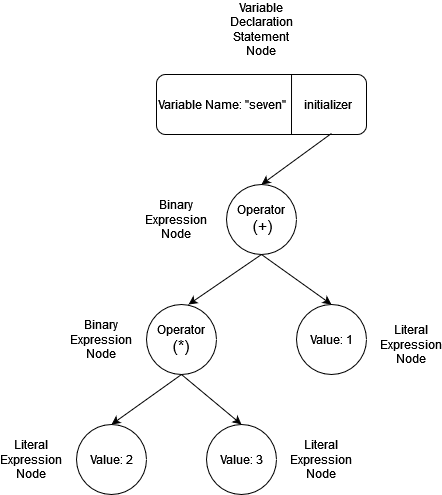
\includegraphics[width=0.6\textwidth, height=0.6\textheight, keepaspectratio]{Figures/Arquiteturas/ParserOutput.png}  
  \caption{Example of AST generated as output by the parser.}
  \label{fig:CompilersAndInterpreters}
\end{figure}

\subsection{Static Analyzer}
The Static Analyzer is the third component present in the compiling process of a compiler. It is responsible for performing a task called static analysis. Static analysis essentially means examining the source code without executing it, hence the name. Delving into it, the static analyzer's task is certify that the source code stick to correctness rules defined by the source programming language design and principles.

Such correctness rules include and are not limited to:
\begin{itemize}
    \item \textbf{Scope and Name Resolution:} This set of rules is responsible for ensuring that variables, functions and classes/types are declared before they are used. In addition, it is also in charge of making the correct bindings between an identifier use and its corresponding declaration, considering the scopes presented in the program's source code.
    
    \item \textbf{Type Checking:} Is an action performed by the static analyzer responsible for ensuring that functions, expressions and variables are properly used. For example: a value of type \texttt{int} cannot be multiplied by a value of type \texttt{bool}, if in a certain function with one parameters expects a value of type \texttt{string}, a value of type \texttt{int} cannot be passed as an argument in a call to such function.
    
    \item \textbf{Detection of Syntax Errors:} Although the parser is responsible for detecting such class of errors, some of these are easier detected during the static analysis stage. For example, a static analyzer can easily detect the misuse of the \texttt{return} keyword outside of a function (default or anonymous) or method. It can also detect the misuse of the \texttt{break} and \texttt{continue} keywords outside of loop statements. There are more examples related to these types of scenarios, but the two mentioned above are good and common examples.
    
    \item \textbf{Detection of Undeclared Variables and Functions:} As the rule's name suggests, a static analyzer is capable of recognizing the usage of variables and functions that have not been previously declared by the developer. It is also worth mentioning, that certain static analyzers take a step beyond and warn the user about variables and functions that have been declared but were never used in the program's source code.
\end{itemize}

Moreover, it is very important to remember the reader that the enforcement of such rules are performed on the Abstract Syntax Tree (AST) provided by the parser in the previous compiling stage, and the output of the static analyzer component is the same, the Abstract Syntax Tree (AST).

Finally, yet importantly, it is essential to highlight the fact that in mature compilers (Clang, GCC, javac, Roslyn, rustc, etc.) there is usually more than one static analyzer component where each one of them is responsible for receiving different representations of the program's source code and, consequently, enforcing different types of rules according to the philosophy of the source language.

For instance, there are static analyzers that are able to identify unused variables from just traversing the generated AST from the parser.

Last but not least, there are static analyzers that only operate on certain representations of the user's source code. Some static analyzers operate on Intermediate Representation (IR), which is a different type of representation of the source code. It is worth mentioning that this one is more abstract and it is designed to be easier to analyze compared to an AST as it removes details that are too specific of the source programming language. Analyzers that act on this type of representation can perform more complex analysis, such as Control Flow Analysis (whose focus is on detecting unreachable code and ensuring the non existence of infinite loops) and Data Flow Analysis (whose focus is on tracking how values flow between variables).

\subsection{Intermediate Representation (IR) Generator}
After the previous phases, it is time for the IR generator comes into play. This component receives as the AST from the Static Analyzer and transforms it into another representation of the user's source code that is generally closer to machine-code or bytecode, which, by consequence, makes it also closer to the hardware.

Before explaining with more details what an IR really is and how it works it is essential to remind the reader that the compiler is divided into two big components: the front-end (responsible for dealing with the source programming language) and the back-end (responsible for dealing with the target computer architecture).

Given this structure, there usually exist some kind of code representation that works as a bridge between the front-end and the back-end. Given this motivation, the IR normally is not tied neither to the source programming language and nor to the machine-code of the target architecture or bytecode. By using an IR to link the front and back-ends, the user can implement multiple compilers targeting different architectures with less effort.

The image below shows the huge different that the use of an IR generator component makes inside a compiler:

\begin{figure}[H]  
  \centering
  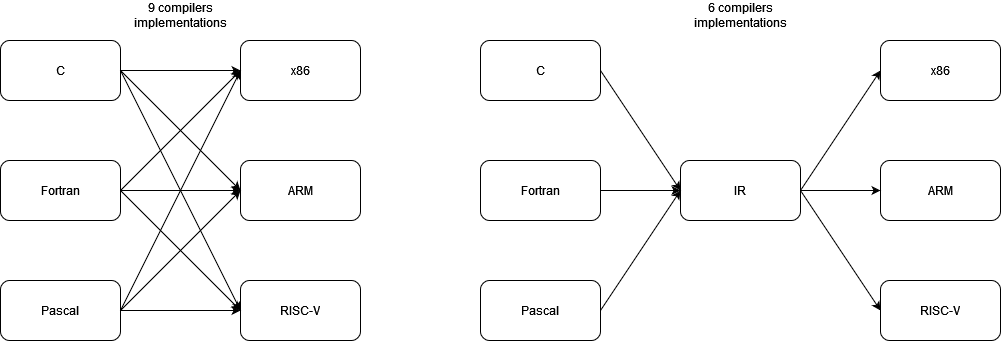
\includegraphics[width=\textwidth, height=\textheight, keepaspectratio]{Figures/Arquiteturas/IRImpact.png}  
  \caption{Impact of IR in multiple compilers implementations.}
  \label{fig:IRImpact}
\end{figure}

Basically, the developer implements only one front-end for each source language that produces the IR. Then only one back-end for each target architecture. Now, one is able to combine those to get every possible combination of source language and target architecture.

\subsection{Optimizer}
After the previous component emits the code in the intermediate representation (IR) format, it is time for the compiler to make the program more efficient in terms of execution time and memory usage without changing the meaning of the program (i.e., its semantics). For that purpose, the optimizer component comes in.

Before providing an overview of optimization techniques, it is important to inform the reader that this subfield of programming languages design and compilers implementation is still very active, with new discoveries and improvements being made in a regular basis. Therefore, this subsection will focus on the most well-known and popular optimization techniques.

Optimization techniques can be divided into two different groups: Machine-Independent Optimization Techniques and Machine-Dependent Optimization Techniques. The first group consists of techniques that can be applied to the user's program in the IR format, this is why they are called machine-independent. The second group is made of optimization techniques that require information about the target hardware architecture in order to be applied, hence the name machine-dependent.

Now, it is time to take a look at these two groups in more details:

\begin{itemize}
    \item \textbf{Machine-Independent Optimization Techniques:}
        \begin{enumerate}
            \item \textbf{Constant Folding:} This optimization consists of checking whether there is an expression in the code that always evaluate to the same value. If that is the case, then, the compiler can perform such evaluation at this stage and replace the code related of the expression with the computed resulting value.
            
            \item \textbf{Constant Propagation:} This technique is responsible for identifying constants in the code and then replacing the use of such constants with their respective values throughout the code.
            
            \item \textbf{Common Subexpression Elimination (CSE):} The aim of this optimization is identify expressions that are computed several times with the exact same operands inside the code and, then, replace all of them with a single computation, making the program faster by not requiring the computation of the same expression multiple times.
            
            \item \textbf{Dead-Code Elimination:} This optimization technique aims to eliminate code that has no effect on the behavior of the program, such as: declared variables that are not used and code placed after a \texttt{return} statement. 
            
            \item \textbf{Inlining:} This one's goal is to remove function calls from the program and include the body of the function where the call to such function was made. By doing this, the overhead related to a function call is reduced, making the program faster.
            
            \item \textbf{Loop Invariant Code Motion:} This optimization technique, as the name suggests, move operations that generate the same result in every iteration of a loop to the outside of it. By performing this action, redundant computations are eliminated, making the program run faster.
            
            \item \textbf{Strength Reduction:} Such optimization approach is responsible for replacing expensive operations, from a computation point of view, with cheaper ones that do not alter the program's behavior.
        \end{enumerate}
    \item \textbf{Machine-Dependent Optimization Techniques:}
        \begin{enumerate}
            \item \textbf{Instruction Scheduling:} This optimization consists of reordering instructions of a particular CPU architecture in order to make a better usage of its instruction pipeline and avoid possible stalls. This sort of optimization takes into account the latency of each instruction and also the availability of finite physical resources, such as registers.
            
            \item \textbf{Register Allocation:} This optimization is responsible for improving the assignment process of variables and produced temporary values to the limited amount of registers from a CPU. Since a CPU has a limited number of registers, this optimization tries to find out which variables and values should be kept in registers and which should be stored in memory, with the purpose of enhancing the performance of the program (it is worth remembering the reader that an access to a register is faster than the access to the memory). Therefore, it is essential to find out which variables and values are more used in the program and store them in registers instead of the memory.
            
            \item \textbf{Instruction Selection:} The goal of this optimization technique is, given the IR representation of the source code, choose the most efficient set of instructions from the target hardware architecture to perform the required operations.
            
            \item \textbf{Branch Prediction Optimization:} This optimization's objective is alter the code configuration in order to minimize the probability of a branch misprediction occurs. Normally, this is achieved by rearranging the code in such way that execution paths that are frequently executed are placed closer and also in a way that matches the CPU's prediction policy.
            
            \item \textbf{Vectorization:} This technique's purpose is convert scalar instruction into vector instructions in order to leverage the SIMD (Single-Instruction, Multiple Data) capabilities of modern CPUs. By doing this, the execution time of the user's program is usually reduced.
        
        \end{enumerate}
\end{itemize}

Finally, as seen above, there are two different groups of optimizations that a compiler can perform. Therefore, it is very common that the pipeline of a compiler has two different optimizers, one right after the IR Generator (that deals with machine-independent optimizations) and another right after the Code Generator (responsible for machine-dependent optimizations).

\subsection{Code Generator}
Once the compiler has performed the machine-independent optimizations to the adopted IR, it is time to generate code for the target CPU architecture. This task is executed by the Code Generator component.

In this context, it is important to highlight to the reader that the generated code is just Assembly code of a specific hardware architecture, whether it is x86, ARM, MIPS, RISC-V or another.

When it comes down to the implementation of this component, two possible paths can be taken by the implementer: one can generate code for an existing architecture, that is a real CPU, or for a virtual one.

If the first way is taken, then the compiler generates machine code for a real CPU and, after that, an executable is yielded and, finally, can be load into the memory of the system by the operating system. The advantage of this approach is that the native code generated is extremely fast since it leverages the most of the architecture that it is targeting. However, the downsides might be intimidating, in order to achieve such speed, one often needs to have a deep knowledge about the architecture that the implemented compiler has selected. Also, once the selection is made, the compiler is tied to such architecture. This means that, if the compiler targets the RISC-V architecture, then it cannot work on a x86 or ARM device.

According to \cite{nystrom2021crafting}, as a mean to deal with these disadvantages, Martin Richards and Niklaus Wirth developed their compilers to generate code for a virtual machine, instead of a real one. In practice, this means that their compilers produced code for an hypothetical and idealized machine rather than for a specific real CPU chip.

Advancing into this topic, the intention behind designing these synthetic instructions of a virtual machine is very clever: It allows the compiler developer to create instructions that are linked to the semantics of the source programming language without needing to worry about the peculiarities of any CPU architecture.


\subsection{Virtual Machines}
As seen above, a virtual machine is one of the possible approaches when it comes to the code generation phase of a compiler.

If the developer has chosen to built a compiler that emits bytecode, then there is still one task left to be done. Since, the compiler yields bytecode, no CPU architecture is able to understand what this representation actually means.

In this case, there are two options available again:
\begin{itemize}
    \item Implement a "mini-compiler" that performs a translation between the generate bytecode and the target machine architecture. In this scenario, it is important to pay attention to two facts: First, the produced bytecode will be essentially acting as a sort of intermediate representation since a translation between it and the target chip will need to happen. Second, the developer is again tied to the underlying hardware architecture. For each computer architecture, a new "mini-compiler" will have to be constructed.
    
    \item Implement a Virtual Machine (VM). In simple words, this is a program that emulates a chip that is able to fully understand the bytecode generated by the compiler. As one can already infer, virtual machines have their own trade-offs. Executing bytecode in a virtual machine is slower than directly executing native code in a computer architecture, due to the fact that each bytecode instruction must be simulated in software every time it executes instead of being executed by the hardware itself. On the other hand, by implementing a virtual machine, one gains a lot in terms of simplicity and portability. The need to translate the bytecode generated by the compiler to the machine code of a certain architecture is eliminated and say that the virtual machine was implemented in C or C++, then the implemented programming language can run in any platform that has a C or C++ compiler installed in it.
\end{itemize}


\subsection{Runtimes}
If the developer has opted to make the code generator directly produce machine code for a certain computer architecture, then the last step is tell the underlying operating system of the computer to load the executable file in the memory and execute it.

On the other hand, if the developer has opted to make the code generator yield bytecode, than the last step is start up the virtual machine, send the generated bytecode to it and execute the VM program.

In both of the mentioned cases, there is usually a need to have an environment that whose responsibility is provide support while the program has started its execution. Such piece of software is an essential part of the programming language implementation called Runtime.

The amount and type of responsibilities assigned to a runtime often varies according to the nature of the implemented programming language. However, some responsibilities are the same across different types of 
programming languages:

\begin{itemize}
    \item Interface with the Operating System.
    \item Memory Management.
    \item Execution of Built-In Functions.
    \item Process and Thread Management.
    \item Type Checking (for Dynamically-Typed Languages).
\end{itemize}


\section{Shortcuts and Alternate Routes}
This section is dedicated to present an overview of a few alternate ways of implementing a programming language besides the structured route exposed in the previous section. 

This is by no means an exhaustive list of possible approaches to be taken. Instead, it provides an overview of the most common and simple ones.

\subsection{Single-Pass Compilers}
A single-pass compiler is simple type of compiler that operates by interleaving the parsing, static analysis and code generation steps inside the parser component in order to generate the output code.

These kinds of compilers function without ever needing to use an AST or another sort of IR.

This simplicity, however, comes with a cost. The language design becomes severely restricted due to the way a single-pass compiler works. The developer does not have any kind of data structure to store information about the program and once some part of the code is parsed, it won't be re-visited later on, hence the name single-pass compiler. Essentially, this means that every time a statement or expression is parsed, the compiler needs to have enough information in order to correctly compile it.

The technique that enables single-pass compilers is known as "syntax-directed translation". In this approach, the developer establishes a link between a component of the programming language's grammar, one that outputs code, and an action to be executed. Then, when the parser starts its job, as soon as it identifies a piece of grammar that has an action associated, it executes such action, emitting the output code, step by step.

According to \cite{nystrom2021crafting}, both C and Pascal were firstly designed with the mentioned limitation in mind. It is worth remembering the reader that, at the time of these languages' conception, memory was very scarce. At certain times, compilers were not even able to deal with a single source file, let alone an entire program.

\subsection{Tree-Walk Interpreters}
A tree-Walk interpreter is a simple kind of interpreter that usually works by executing code right after the parser generates the AST.

In this scenario, a tree-walk interpreter runs the user's source code by executing a traversal on the received AST and performing different types of actions by taking into account the type of node that it is currently on.

Due to its simplicity, this kind of programming language implementation is very common in student projects and educational programming languages. However, it is not often used in general-purpose language, since the nature of the code execution makes it slow, with one exception, according to \cite{nystrom2021crafting}, being the earlier versions of Ruby, which were implemented as tree-walk interpreters up to version 1.9, when the language implementation was changed to a bytecode virtual machine.

\subsection{Transpilers}
A transpiler, also known as source-to-source compiler or transcompiler, is special type of compiler. The idea behind it is very simple: Instead of translating the program written in a source programming language to some kind of intermediate representation (AST, IR, CFG, etc), it translates the program to another source programming language.

Going further into its functioning, the developer writes the front-end components of a compiler as usual. Nevertheless, in the compiler's back-end, the programmer generates a string of valid code in another programming language that is as high-level as the source language, while preserving the meaning and semantics of the original program.

Finally, the programmer can use the compiler for the chosen high-level target language in order to delegate the heavy lifting of the back-end stage to this compiler. 

One of the most common use cases of a transpiler occurs in the context of web browsers. Nowadays, JavaScript is, by far, the most common choice to run code in it. However, JavaScript might not provide the best coding experience from certain developers' point of view. Due to that, a growing increase in the number of transpilers that have JavaScript as their target language has been observed, as can be seen in \cite{coffeescriptCompileToJS}.

\chapter{Context and Purpose} \label{cap:metodologia}

\begin{displayquote}
    \begin{center}
        \textit{``I wonder if I can keep up with... the speed of a world you're not in.''}
    \end{center}
\end{displayquote}

\begin{flushright}
   \textit{-- NORIAKI KUBO}
\end{flushright}

\section{Introduction}
This chapter is dedicated to provide the historical context on how the way of teaching undergraduate Compilers courses evolved since the 70s, as well as a brief overview of surveys that demonstrate the positive impact that more practice-orient approach brings to students. Such factors are what motivated the creation of the Bleach programming language. Furthermore, a revisit and deepening regarding the purpose of Bleach is also. Then, an analysis about how Bleach distinguishes itself from other proposed programming languages that also aim to be used in Compiler courses is presented. In the end, the chapter provides a detailed description about the context Bleach is inserted in, which includes: the target audience, educational environment, typical use cases and the educational benefits provided by it.

\section{Historical Evolution of Compilers Courses}
Looking back at the history of compiler construction \cite{wikipedia_compiler_construction} and the history of programming languages \cite{wikipedia_programming_languages}, it can be said that the way of teaching an undergraduate Compilers course evolved as follows.

During the 1970s, undergraduate Compilers courses used to have a heavy focus on the theoretical aspects of the field, such as formal languages, automata theory, lexing techniques and parsing techniques. During that period, access to computational resources were still scarce, even in an academic environment. However, students were still able to implement toy compilers in different tastes of Assembly or in an early high-level language like Fortran \cite{fortran_official_website}. Still, the pillars of this course emphasized a deep understanding of the theoretical and formal aspects mentioned above.

In the 1980s, even though the focus of these courses remained rooted in theoretical aspects (lexical analysis, syntax analysis and the fundamental of code generation and optimization), a gradual shift from theory to practice started to happen. Thanks to the spread of languages like C \cite{kernighan1988c}, C++ \cite{strousrup2000c++} and Pascal \cite{wirth1971programming}, more practical implementations of compilers were allowed to be made. Therefore, courses started to add more practical projects. In such projects, students were usually asked to write a compiler (or parts of one) in these new languages. Last, but not least, the rise of UNIX \cite{ritchie1978unix}, Lex \cite{lesk1975lex} and Yacc \cite{johnson1975yacc} allowed students to implement components of a compiler with more ease. This improvement led to more sophisticated course projects.

In the 90s, such courses had already become more oriented to hands-on experience thanks to the improvements achieved in the previous decade. The birth of languages like Java \cite{java_17_official_specification} and the increase in computational power of personal computers allowed students to tackle more complex compiler projects. Courses started to assign to students more complicated tasks like the implementation of entire compilers for small languages or significant compiler components, such as code generators and optimizers. Moreover, the textbook \cite{aho1986compilers}, popularly known as "The Dragon Book", became the standard reference in this field.

In the 00s, this trend of giving more focus to the practical experience went on, with a focus on real-world applications and the use of modern programming languages. Furthermore, courses began to add more advanced topics to their syllabus, such as just-in-time compilation, garbage collection, and runtime environments. It's safe to say that the way of teaching Compilers became more holistic, covering not just compiler theory and implementation but also language design and performance optimization. During this period, Alfred Aho published \cite{aho2008teaching}, an article in which he reflects on how the way of teaching undergraduate Compilers courses has evolved through the years and also how he changed his way of teaching such course. According to him, it is still possible to teach it in a way that provides educational benefits and satisfaction to the students. The latest approach adopted by him consisted on presenting the basics of the most important topics (lexical analysis, parsing, semantic analysis, intermediate code generation, runtime environments, resource management and target code generation). At the same time, Aho asked his students to implement a compiler and provided the specifications of the source and target languages for the compiler they were implementing. He also noticed that the students weren't excited about implementing someone else's language. Thus, he took a bold move and assigned his students the task of working in smalls team to define their own
language and then build a compiler for it. Such approach, according to him, made the students much more engaged and excited.

Finally, in the 2010s and 2020s, the teaching of this course continued the trend of emphasis on balancing theory and practice. Such factor influenced the way Compilers course were taught, as professors and instructors began to integrate more diverse and flexible learning materials, including video lectures, interactive simulations, and online coding platforms. Also, the COVID-19 pandemic played an important role in this change, since it forced educators to rethink how compilers could be taught in a remote manner, which led to rise of new assisting tool like virtual laboratories, collaborative coding environments and online assessment tools. Consequently, such courses became more modular, allowing students to learn at their own pace and apply their knowledge in a way that felt meaningful to them.

\section{Reports on More Practical Ways of Teaching Compilers Courses}
In this section, a few reports that discuss different approach to teach an undergraduate Compilers course are presented, along with their main findings.

In 2015, Lasseter \cite{lasseter2015interpreter} proposed a new strategy to present the fundamental concepts of an undergraduate Compiler Construction course. The suggested approach defends that the concept of an Interpreter serves as an effective conceptual framework that can be used to educate students about the later stages of the compilation pipeline, specially the semantic analysis and code generation phases. As reported by the author, this line of action is useful in the way that it not only unifies the major theoretical concepts of this undergraduate course, but is also helpful when it comes to the implementation of semester-long compiler construction project. At Hobart \& William Smith Colleges, the university where Lasseter works, the undergraduate Compiler Construction course is a one-semester, upper-division elective, offered every other year. The course addresses both software engineering aspects as well as the major concepts of a traditional Compilers course (lexing, parsing, semantic analysis and code generation). Moreover, it already adopts a more practice-oriented approach where every student must present a working compiler by the end of the 15-week semester. When it comes to the course project itself, Lasseter opted to use the Tiger programming language \cite{appel1998tiger}, originally developed by Andrew Appel for his project-oriented "Modern Compiler Implementation" suite of C, ML and Java textbooks \cite{appel1997modernCompilerImplementationC}, \cite{appel2002modernCompilerImplementationJava}, \cite{appel2004modernCompilerImplementationML}. During the years in which the author was responsible for this course, he noticed a worrying pattern: Even though the students did well in the first stages of compilation (lexing and parsing), the vast majority of them started to struggle with the semantic analysis stage. According to the students, the combination of the underlying concepts of type checking, the details of the famous visitor pattern when traversing an AST and the interaction between this design pattern and a real-world semantic analysis implementation is just too overwhelming. Given this scenario, Lasseter chose to schedule individual meetings with this students where he introduced the idea of a language's interpreter as a touchstone to better explain the last two stages of the compilation pipeline. His investigation led to the fact that such approach proved to be the to be most uniformly effective among the students with whom he discussed. In light of this discovery, professor Lasseter reorganized his lectures introducing these specific compiler phases to include the interpreter structure as a reference point. Finally, he came to the conclusion that adding lectures that presented the concepts behind the interpreter framework resulted on better understanding of the students when it came down to the semantic analysis and code generation phases of the compilation process, indicating that the idea of an interpreter has a substantial educational value in this field.

In 2016, Kundra et al. \cite{kundra2016experience} proposed a novel approach called "Case-based and Project-based Learning" to teach a Compilers Design course to B.Tech third year students of a Delhi University (India) college. The responsibles for implementing such methodology based themselves in the definition of what is Traditional Learning present in \cite{altman2010workplace} and used the definition and core ideas of Case-based Learning present in \cite{golich2000abcs} in order to propose their own method. According to the authors, this proposed method combines 4 different pedagogical models, which makes this approach unique and effective: Didactic Teaching \cite{altman2010workplace}, Problem-Based Learning \cite{hmelo2004problem}, Cognitive Apprenticeship Model \cite{dennen2008cognitive} and Project-Based Learning \cite{thomas2000review}. To implement it, they divided one core project of this class into several sub-projects with the goal of improving the practical experience of the students when it came down to the task of designing a compiler. To evaluate the effectiveness of this approach, students were asked to complete a survey that grasped on their perceptions about the upsides of such method. Such survey was analyzed using the following statistical tools: frequency estimation and chi square test of association. According to the paper, the results showed that the proposed approach indeed had a positive impact on students since it enhanced their learning, critical thinking, engagement, communication skills and team work. In the end, the authors came to the conclusion that the outcome of the survey analysis proved that both Case-based and Project-based learning are suitable for teaching concepts of compilers implementation.

In 2021, Robert Nystrom, a software engineer that works at Google on the Dart language, published the "Crafting Interpreters" book \cite{nystrom2021crafting}: An extensive guide about not only implementing two different types of interpreters for Lox, a full-featured programming language designed by the author, but also a walkthrough that guides the readers on how they can design their own programming language. The book assumes that its the reader first contact with this field. Therefore, it covers each concept needed in an approachable style while also providing every line of code needed to implement the two types of interpreters covered. As the author himself admits in the first chapter of the book, "Crafting Interpreters" is not meant to be as rigorous as other references, such as \cite{aho1986compilers} or \cite{cooper2022engineering} when it comes to the theoretical foundation of programming languages. Instead, as suggested earlier, its purpose is to be lighter in theory, while still introducing the history and core concepts of programming languages implementation. Moreover, the author stands by the point of view that the best way of learning a new subject is by practicing and experimenting. He even says that his goal is that every reader finish his book with a solid intuition about how real programming languages work. The book also aims that the reader will feel more comfortable when reading more advanced and theoretical books later on, such as \cite{aho1986compilers}, \cite{cooper2022engineering} or \cite{muchnick1997advanced}. It's important to keep in mind that the book's focus is on building interpreters, which are simpler and more accessible to understand when compared to compilers. Furthermore, this way of teaching allows the students to have a better comprehension of vital concepts previously mentioned, like lexing/scanning, parsing, abstract syntax trees, semantic analysis and runtime execution without the daunting complexity of optimization and code generation phases that most compilers require. This approach brings a lot of benefits for students and professors. With respect to the students, they are usually able to build a deeper and stronger foundation about how programming languages work since the project-based nature of the book makes them apply what they learn immediately. This solid foundation is, without a doubt, of great use to those who wish to delve deeper into the field. As for the professors, the engaging writing style of the book tends to keep students engaged and motivated during the whole duration of the course, which leads to a better retention and a more rewarding learning experience. Last but not least, it's important to highlight the fact that the "Crafting Interpreters" book is increasingly gaining more popularity and recognition due to its excellence when it comes to conveys the subject of study. It's purchase page on Amazon \cite{nystrom_crafting_interpreters_amazon} is full of reviews praising its quality. Searching for the keywords "crafting interpreters" \cite{crafting_interpreters_repositories_github} shows that there are more than 2600 public repositories implementing the Lox language presented in the book, which is also a testimonial of the popularity and quality of such material.

\section{Revisiting Bleach's Purpose}
As stated in the summary and previous sections of this document, Bleach is a programming language intended to be used as a tool by teachers, instructors and teaching assistants responsible for undergraduate courses in Compilers, ubiquitous in Bachelor's degrees in Computer Science and Computer Engineering.

The inspiration to create Bleach came from the fact that even though there are new approaches that combines theory and practice to expose the contents of the course's syllabus, there are still worrying issues when it comes down to the learning experience of the students, as reported by Lasseter in \cite{lasseter2015interpreter}. With regards to this particular issue raised, the approach proposed by Nystrom in \cite{nystrom2021crafting} seems to be a good and innovative way of teaching Compilers. To reinforce the benefits of a more practical line of action, it's worth remembering that, as seen in the previous section, the "Case-based and Project-based" approach proposed by Kundra et al. in \cite{kundra2016experience} ratifies the idea that a project-based direction for the course is, indeed, a good option when prioritizing the students' experience. On the other hand, such a approach must be executed with carefulness since a similar approach proposed by Aho in \cite{aho2008teaching} may be unfeasible, especially in scenarios where there is a lack of teaching assistants or classes with too many students.

Keeping all of these mentioned points in mind, Bleach aims to be an alternative programming language that seeks to be used in undergraduate Compilers course as a means to engage and motivate students during the learning process of this subject, while also providing enough theoretical foundation for the students in this matter. In addition, it also relieves professors, instructors and teaching assistants from the burden of dealing with dozens of programming languages created by class students.

\section{Existing Toy Programming Languages}

Before taking a deep dive in what makes Bleach an actual and viable option to be used in a classroom environment, it's important to mention that there are several programming languages created with the purpose of being a supplementary tool for teaching undergraduate Compilers course that have opted for a more practice-oriented procedure.

In this section, some of the most popular programming languages designed with this motivation will be discussed in chronological order. The intention with this is to provide information about their origin, historical context and features.

\begin{itemize}
    \item \textbf{COOL (Classroom Object-Oriented Language):} This is a object-oriented and statically-typed programming language \cite{aiken1996cool} created in the 90s by Alexander Aiken and his colleagues at the Stanford University. It was designed with the intention to be used as a tool in an educational setting in universities. Even though COOL is simple and small, it has an interesting variety of features besides the ones mentioned above, such as: basic class types (Bool, Int, IO, Object and String), automatic garbage collection and many others that can be found at "The COOL Reference Manual" \cite{cool_reference_manual}.
    
    According to Aiken, a compiler project is normally the most complex software project that most undergraduate students will complete. Therefore, the use of a full-featured programming language (any language that has a substantial number of users, like C, C++, Pascal, etc) does not fit into the scope of such project. In practice, the usual approach was to select a subset of these popular languages and ask the students to implement them. However, according to Aiken, this method is too demanding for the teaching staff, since several steps must be taken after choosing a language for a Compilers project. For example: a detailed specification of the project itself must be written, any supporting software that might be used must be developed, tested and documented beforehand. Finally, the project itself must also be implemented by the teaching staff \textit{a priori} since, according to Aiken, such effort is required to guarantee that the project is complete, consistent and tractable.
    
    It was with all the efforts mentioned above to build a framework for a compiler project  in mind that Aiken created COOL. Ultimately, it is worth mentioning that COOL is not only a programming language, but rather a freely available and portable compiler project. COOL has being distributed since its creation with the goal of helping professors from other institutions to leverage from the efforts of the project developers and the many students who have written COOL compilers in order to structure their own Compilers courses following their own tastes. COOL has been adopted at several relevant institutions, such as University of California, Berkeley \cite{aiken1996cool} (where it was first introduced), Stanford University \cite{stanford_cs143_compilers_course_page}, University of Illinois Urbana-Champaign \cite{university_of_illinois_urbana_champaign_compilers_course_page} and University of Michigan \cite{university_of_michigan_compiler_construction_course_page}.
    
    \item \textbf{MiniJava:} This programming language \cite{cambridge_minijava_project} is a subset, as its name suggests, of the Java programming language. MiniJava was created by Andrew Appel and Jens Palsberg during the 90s and was first presented as part of \cite{appel2002modernCompilerImplementationJava}. This subset of Java contains its most core features, such as: classes, attributes/fields, methods, logical control structures (if-else) and loop control structures (while). However, since it was tailored for an educational environment, it doesn't contain Java's more advanced features, like: exceptions, generics, inheritance, interfaces and lambda functions. More details about which features MiniJava exactly keeps can be found at \cite{cambridge_minijava_project} and \cite{cambridge_minijava_grammar}.
        
    Its purpose is to be used as a teaching tool in Compilers courses. Since it is a subset, as previously mentioned, it allows the students to focus on the fundamental concepts of this subject without overwhelming them with the complexities of a full-fledged programming language like Java.
    A proof of its success is that MiniJava has been adopted in several prestigious universities worldwide as part of their computer science curriculum, particularly in courses related to compiler construction and programming language implementation, such as University of Washington \cite{university_of_washington_cs_compiler_construction_course_page_2024}, University of California, Los Angeles \cite{ucla_cs_compiler_construction_course_page_fall_2012}, among others, like the Loyola University of Chicago \cite{loyola_university_of_chicago_cs_compiler_construction_course_page_fall_2018}.     
    
    \item \textbf{C* (C Star):} The C* (C Star) programming language \cite{kirsch2017selfie} is a programming language created in 2017 by Christoph M. Kirsch as a component of the Selfie Open-Source Software Project \cite{selfie_official_website} \cite{selfie_official_repo_github}.

    According to Kirsch, the creation of C*, as well as the Selfie project as a whole, was inspired by seminal works made in different sub-fields from Computer Science, such as: Algorithms \cite{knuth2011art} \cite{wirth1976algorithms}, Compilers \cite{wirth1996compiler}, Computer Architecture \cite{hennessy2011computer}, Operating Systems \cite{liedtke1996toward}, Programming Languages \cite{kernighan1988c} \cite{richards2009bcpl}, Systems Engineering \cite{dijkstra1968structure} \cite{goldberg1983smalltalk} \cite{nisan2005elements} \cite{sussman1996structure} and Theory of Computation \cite{sipser1996introduction}. In addition, it was motivated by the challenge of teaching the basics of this field to larger audiences that are not specifically majoring in Computer Science.

    Regarding adoption of C*, the language has been adopted by the University of Salzburg at Austria \cite{selfie_official_website} and by the Czech Technical University (CTU) at Czech Republic \cite{cvut_compiler_construction_course_page}.

    C* has support for 5 different types of statements (assignment, if-then-else, while loop, function call, return). Related to this, the language also implements the following native built-in functions: \texttt{exit}, \texttt{malloc}, \texttt{open}, \texttt{read} and \texttt{write} (it is important to notice the absence of \texttt{close} and \texttt{free}). Regarding to keywords, C* has just 6: \texttt{int}, \texttt{while}, \texttt{if}, \texttt{else}, \texttt{return} and \texttt{void}. Talking about functions, C* allows them to have parameters, local variables and a return value. With respect to operators, C* has support to the most common arithmetic (\texttt{+}, \texttt{-}, \texttt{*}, \texttt{/}, \texttt{\%}) and comparison (\texttt{==}, \texttt{!=}, \texttt{>}, \texttt{>=}, \texttt{<}, \texttt{<=}) operators. However, it does not support bit-wise nor boolean operators. There are just 2 data types present in C*: signed integer (\texttt{int}) and pointer to signed integer (\texttt{int*}). It's worth mentioning that C* has support for integer, character and string literal however. Finally, when it comes to the access of dynamically-allocated memory, the only way of doing so is through the use of the dereferencing operator (\texttt{*}).
    
    \item \textbf{ChocoPy:} ChocoPy is a programming language created in 2019 and first presented at Padhye et al. \cite{padhye2019chocopy} with the goal of being used as a teaching tool in an undergraduate course on compilers and programming language. It is a subset of Python 3.6 that uses static type annotations in order to ensure compile-time type-safety. The project stands out due to its complete specification, which uses a formal grammar, typing rules and operational semantics as described in \cite{padhye2019chocopy}. More technical information about ChocoPy can be found at ChocoPy's official website \cite{chocopy_official_website}.

    According to the authors of \cite{padhye2019chocopy}, the purpose of creating ChocoPy was based on the following 5 major reasons:
    \begin{itemize}
        \item \textbf{Familiarity:} The staff behind the project wanted to develop a language that was a subset of a widely used programming language, hence, prioritizing the familiarity of the students with it. With this reasoning in mind, Python \cite{python_language} was chosen.
        \item \textbf{Expressiveness:} The professionals responsible for ChocoPy wanted to create a language that allowed students to write non-trivial programs in it. Particularly, an Object-Oriented paradigm with enough complexity got chosen to be supported. This option was made in order to illustrate important language implementation concepts, such as optimized code generation and type-checking at compile-time. 
        \item \textbf{Formally Specified:} In order to make a robust tie the theoretical concepts presented in an undergraduate Compilers course with their application in an implementation project, the authors opted for a language whose syntax, type-checking rules and operational semantics were all formally specified. With these needs kept in mind, Python was a good alternative.
        \item \textbf{Modern Target Language:} Instead of targeting an old or too complex Assembly language. Too make the code generation less intimidating, the instructors instead opted for targeting the 32-bits RISC-V Instruction Set Architecture \cite{riscv_instruction_set_manual}.
        \item \textbf{Re-usability:} One of the major reasons for ChocoPy's creation was the democratization of artifacts that could be freely used by professors, instructors, teaching assistants and students from different institutions offering Compilers courses.
    \end{itemize}

    The language started out being used at the UC Berkeley, as stated in \cite{padhye2019chocopy}, and since then has been adopted by several other institutions, such as: TU Delft \cite{tu_delft_cs4200_2020_compiler_construction_course_page}, UC San Diego \cite{uc_san_diego_cse213_winter2021_advanced_compiler_design_course_page} and NYU \cite{nyu_2020_compiler_construction_course_page}. Finally, the ChocoPy language specification was also used as a reference at IIT Bombay \cite{iit_bombay_sclp}.

    As previously stated, ChocoPy was designed to be a subset of Python. In practice, this means that every valid ChocoPy program that does not result in a runtime error is also a valid Python program. Therefore, the result observed when executing the said ChocoPy program is equal to the one when executing the same program in a Python Interpreter. When it comes down to language features, ChocoPy has support for statements, expressions, assignments and control-flow structures (conditionals and loops). When dealing with evaluation of an expression, the result will always have one of the following types: a boolean, an integer, a list, a string, an user-defined class or the special value \texttt{None}. Unfortunately, according to the authors of \cite{padhye2019chocopy}, the language does not have support for dict type, first-class functions and reflective introspection. It is also worth mentioning every expression in ChocoPy is statically typed. On top of it, variables (both global and local ones) and class attributes are also statically typed and have explicit type annotations. Ultimately, type annotations are also present in function and method declarations in order to signal the parameters' and return value's type. More information about ChocoPy's features can be found in \cite{padhye2019chocopy} and in \cite{chocopy_v2.2_language_manual_reference}.
    
\end{itemize}

\section{Scenario Overview}
In this section the context in which Bleach is expected to be used, who will be using it, and how it fits into the educational environment of an undergraduate compilers course are all presented with more details.

\begin{itemize}
    \item \textbf{Target Audience:}
    \item \textbf{Educational Environment:}
    \item \textbf{Use Cases:}
    \item \textbf{Educational Benefits:}
\end{itemize}
\chapter{Bleach} \label{cap:metodologia}

\begin{displayquote}
    \begin{center}
        \textit{``Bullet, Claw, Battle Flag, Short Sword. With my fingers bent, I wait for you.''}
    \end{center}
\end{displayquote}

\begin{flushright}
   \textit{-- TITE KUBO}
\end{flushright}

\section{Introduction}
This chapter is dedicated to provide a detailed explanation about the Bleach programming language. Firstly, a brief overview of Bleach's features will be presented by showcasing a few programs written in the language. Then, a detailed breakdown of each of its components and features will be shown to the reader. Afterwards, the challenges encountered during the development of this project will be presented, as well as decisions and trade-offs made. Finally, a comparison between Bleach and the previous languages introduced will be made, as well as a discussion about how Bleach can be properly used to its fullest in an undergraduate Compilers course.

\section{Bleach Overview}
As previously mentioned, this section is dedicated to showcase a few of Bleach's features through the exposition of simple, yet useful, programs to the reader. It's expected that the reader has some familiarity programming with another languages, such as C \cite{kernighan1988c}, C++ \cite{strousrup2000c++}, JavaScript, Lox \cite{nystrom2021crafting}, Python \cite{python_language} and Ruby, so the similarities between Bleach and these languages make themselves more evident. \newline

\begin{figure}
    \centering
    \begin{lstlisting}
function greet(){
  print "Hello, World!";
}

greet(); // "Hello, World!"
    \end{lstlisting}
    \caption{Bleach's simplest program: The famous "Hello, World!" program.}
\end{figure}

\begin{figure}
    \centering
    \begin{lstlisting}
function factorial(n){
  if(n == 0){
    return 1;
  }else{
    return n * factorial(n - 1);
  }
}

print factorial(5); // 120
    \end{lstlisting}
    \caption{A Bleach program that shows the usage of recursive functions, if-else statements and arithmetic operators to calculate the factorial of a number.}
\end{figure}

\begin{figure}
    \centering
    \begin{lstlisting}
function main(){
  let numbersInfo = [];
  for(let i = 0; i <= 10; i = i + 1){
    if(i % 2 == 0){
      numbersInfo.append(i + " is even!");
    }else{
      numbersInfo.append(i + " is odd!");
    }
  }
  print numbersInfo;
}

main();
    \end{lstlisting}
    \caption{A Bleach program that shows the usage of for loops and the native \texttt{list} type in order to build a list that contains some information about numbers from 0 to 10.}
\end{figure}

\begin{figure}
    \centering
    \begin{lstlisting}
function quadraticEquationSolver(a, b, c){
  let delta = std::math::pow(b, 2) - 4 * a * c;
  let x1 = (-b + std::math::sqrt(delta))/(2 * a);
  let x2 = (-b - std::math::sqrt(delta))/(2 * a);

  return [x1, x2];
}

print quadraticEquationSolver(1, 0, -4); // [2, -2]
    \end{lstlisting}
    \caption{A Bleach that uses a function which receives the coefficients of a quadratic equation to compute its roots.}
\end{figure}

\begin{figure}
    \centering
    \begin{lstlisting}
class Shape{ // Base Class
  method init(name){
    self.name = name;
  }

  method str() {
    return "This is a " + self.name + ".";
  }

  method area(){ // To be overridden by subclasses
    return 0;
  }
}

class Circle inherits Shape{ // Derived Class
  method init(radius){
    super.init("Circle"); // Call the Base Class constructor
    self.radius = radius;
  }

  method area(){
    return std::math::pow(self.radius, 2) * 3.14159;
  }
}

class Triangle inherits Shape{ // Derived Class
  method init(base, height) {
    super.init("Triangle"); // Call the Base Class constructor
    self.base = base;
    self.height = height;
  }

  method area(){
    return (self.base * self.height) / 2;
  }
}

let c = Circle(5);
let t = Triangle(3, 7);

// This is a Circle. It has an area of 78.539749999999998 units.
print c + " It has an area of " + c.area() + " units.";
// This is a Triangle. It has an area of 10.5 units.
print t + " It has an area of " + t.area() + " units.";
    \end{lstlisting}
    \caption{A Bleach program that illustrates its Object-Oriented features, such as: classes, instances, attributes, methods, overriding and inheritance.}
\end{figure}

\begin{figure}
    \centering
    \begin{lstlisting}
function writeToFile(){
  let userInput = std::io::readLine();
  std::io::fileWrite("output.txt", "w", userInput, true);

  userInput = std::io::readLine();
  std::io::fileWrite("output.txt", "a", userInput, false);

  return;
}

writeToFile();
    \end{lstlisting}
    \caption{A Bleach program that shows its capability with dealing with user-input and writing to \texttt{.txt} files.}
\end{figure}

\section{Bleach Features}
\subsection{Introduction}
This section, as its name suggests, is dedicated to provide to the reader a more extensive and exhausting walkthrough the features available in Bleach. 

\subsection{Data Types}
Bleach has 5 built-in data types made available to the user. Such types are divided into scalar types  and compound types.

Scalar types are types that can represent a single value. In Bleach, there are 3 scalar data types: \texttt{bool}, \texttt{nil} and \texttt{num}.
\begin{itemize}
    \item \texttt{bool}: This data type is used to represent one of two possible values: \texttt{true} or \texttt{false}. Such values are used to express logical conditions and to control the execution of certain parts of a program's source code.
    
    In this context, it's important to mention that Bleach takes inspiration from Ruby and other modern programming languages and implements the concept of "truthy" and "falsey" values in order to evaluate the truthiness or the falseness of values when they are being evaluated inside \texttt{if} statements, loops (\texttt{while}, \texttt{do-while}, \texttt{for}) and ternary operators (\texttt{? :}).

    Essentially, this means that, in Bleach, values of any type (built-in or user-defined) can be used in places where a value of type \texttt{bool} is expected. Moreover, Bleach opted to follow the same convention of Ruby in this matter, which says:

    \begin{itemize}
        \item \textbf{"Falsey" values:} \texttt{false}, \texttt{nil}.
        \item \textbf{"Truthy" values:} Any other value that is not \texttt{false} nor \texttt{nil}.
    \end{itemize}
    
    \item \texttt{nil}: This one is an old acquaintance for most programmers. The \texttt{nil} type has just one possible value: the \texttt{nil} value. In short this value conveys the idea of "no value" or the idea of "absence of a value".

    In other programming languages, this concept appears in other forms, like: \texttt{NULL}, \texttt{nullptr}, \texttt{null}, \texttt{None}, \texttt{nil}, and others. Since Bleach has some influence from Ruby, it adopted \texttt{nil}.
    
    \item \texttt{num}: In favor of simplicity, Bleach has only one type to represent numbers: the \texttt{num} type. This type can be used to represent both integers and floating-point numbers.

    Behind the scenes, the \texttt{num} type is implemented with a double-precision floating-point type, which allows Bleach to cover a lot of territory when it comes to numerical values while still keeping the simplicity initially envisioned for the language.
    
    Finally, with respect to numerical literals, Bleach has support for only basic integer and decimal literals, such as: \texttt{23}, \texttt{42}, \texttt{3.14159}, \texttt{2.71828}, \texttt{-10.4}.
    
\end{itemize}

Compound types are types that can group multiple values into one. In Bleach, there are 2 compound types: \texttt{list} and \texttt{str}.
\begin{itemize}
    \item \texttt{list}: Taking inspiration from Python \cite{python_language}, Bleach has this type. Here, the \texttt{list} type represents an linear-sequence of elements. As previously stated, Bleach is a dynamically-typed language, just like Python. Thus, the \texttt{list} type can store values of different types with no issues. Moreover, Bleach has support for \texttt{list} literals, just as the ones shown below:\newline

    \begin{figure}[H]
        \centering
        \begin{lstlisting}
let l0 = [0, 1, 2, 3, 2.71, 3.14159];
let l1 = ["hello", "there"];
let l2 = [];
let l3 = [false, "Brazil", 9.98, nil];
        \end{lstlisting}
        \caption{Examples of \texttt{list} literals in Bleach.}
    \end{figure}

    Finally, as in Python, the \texttt{list} type in Bleach has the following useful methods that makes the student's life easier when working with this type.
    
    \begin{itemize}
        \item \texttt{append}: Method responsible for adding one value of any type to the end of the \texttt{list} value it was called on. Returns \texttt{nil}.
        \item \texttt{clear}: Method responsible for deleting every element that is currently stored inside the \texttt{list} value it was called on. Returns \texttt{nil}.
        \item \texttt{empty}: Method responsible for checking whether the \texttt{list} value it was called on currently has values stored inside it or not. Returns a \texttt{bool} value.
        \item \texttt{fill}: Method responsible for resizing the \texttt{list} value it was called on to a provided size and also filling all of its indexes with a provided value of any type. Returns \texttt{nil}; 
        \item \texttt{getAt}: Method responsible for returning the value present at the provided index. Returns a value of any type.
        \item \texttt{pop}: Method responsible for deleting and returning the last element present inside a \texttt{list} value, if any. Returns a value of any type.
        \item \texttt{setAt}: Method responsible for setting the value stored at the provided index to the value that was provided. Returns \texttt{nil}.
        \item \texttt{size}: Method responsible for checking and returning the current amount of elements that the \texttt{list} value it was on called on currently has. Return a \texttt{num} value.
    \end{itemize}

    Last but not least, it's important to mention that any misuse of the methods presented above will result in a runtime error during the program's execution.

    \item \texttt{str}: Also taking inspiration from Python \cite{python_language}, Bleach has this type. The \texttt{str} type represents an indexed-sequence of characters (a string), typically used to store and manipulate text. Just as the \texttt{list} type, Bleach also has support for literal values of this type:

    \begin{figure}[H]
        \centering
        \begin{lstlisting}
let s0 = "Ichigo Kurosaki";
let s1 = "Byakuya Kuchiki";
let s2 = "Bazzard Black";
let s3 = "Jugram Haschwalth";
        \end{lstlisting}
        \caption{Examples of \texttt{str} literals in Bleach.}
    \end{figure}

    There are other aspects about the \texttt{str} type that must be mentioned.

    First of all, it is important to recall that it's a sequence type. In short, it means that values of this type can be indexed. In a string, indexing usually allows the programmer to access individual characters from the value, which, in the Bleach programming language, are also values of \texttt{str} type.

    Also, as seen in Figure 4.8, in Bleach, literals values of this type are always enclosed by double quotes (\texttt{""}).

    Finally, as in Python, this type has the following useful methods available:

    \begin{itemize}
        \item \texttt{empty}: Method responsible for checking whether the \texttt{str} value it was called is equal to \texttt{""} or not. Returns a \texttt{bool} value.
        \item \texttt{find}: Method responsible for trying to figure out if the provided sub-string (a \texttt{str} value) exists within the \texttt{str} value the method was called on. Returns a \texttt{num} value which denotes the index at which the sub-string appears, otherwise returns \texttt{-1}. 
        \item \texttt{length}: Method responsible for checking and returning the current amount of characters (which are also values of type \texttt{str}) that the \texttt{str} value it was on called on currently has. Returns a \texttt{num} value.
        \item \texttt{split}: Method responsible for generating a \texttt{list} where each value is of \texttt{str} type. This method receives as its unique argument a value of \texttt{str} type that works as the separator. Returns a \texttt{list} value.
        \item \texttt{substr}: Method responsible for retrieving a sub-string from the \texttt{str} value it was called on. The method receives two arguments of \texttt{num} type that work as the start and end delimiters. Returns a \texttt{str} value.
    \end{itemize}

\end{itemize}

\subsection{Comments}
Even though it is recommendable that a programmer writes code in a way that is readable and understandable, there are certain scenarios where extra explanation about what certain parts of a program's source code is actually doing is necessary.

In these specific cases, programmers usually leave comments in their code that the compiler/interpreter will ignore but people reading their code may find helpful.

Given this, Bleach takes inspiration from C \cite{kernighan1988c} when it comes to support for single-line comments and multi-line comments.

\begin{itemize}
    \item \textbf{Single-Line Comments:} In Bleach, a single-line comment starts with two slashes (\texttt{//}), and the comment continues until the end of the line.
    \item \textbf{Multi-Line Comments:} Bleach also has support for multi-line comments. A multi-line comment has a beginning and an ending. The former is denoted by a (\texttt{/*}), while the later is denoted by a (\texttt{*/}). Everything written in-between is considered a comment and, thus, is ignored by the interpreter at runtime.
\end{itemize}

    \begin{figure}[H]
        \centering
        \begin{lstlisting}
// This is a single-line comment.

/*
This 
is
a
multi-line
comment.
*/
        \end{lstlisting}
        \caption{Examples of \texttt{str} literals in Bleach.}
    \end{figure}

\subsection{Variables}
A variable, as in most programming languages, can be viewed as just a name associated with a storage location in memory. Such storage location is responsible for holding data that can be changed during the execution of a program.

In Bleach this is not different. Variables still have this main functionality. However, they have some particularities that might differ from variables in other programming languages. Such peculiarities are listed below:
\begin{itemize}
    \item In Bleach, all variables are mutable. In other words, once a variable is declared, any amount of assignments are allowed to be performed on this declared variable.
    
    \item A direct consequence of the particularity explained above is that there is no concept of constants in Bleach. There are just mutable variables, as previously mentioned.
    
    \item In Bleach, to declare a new variable, the \texttt{let} keyword must be used:
    \begin{figure}[H]
        \centering
        \begin{lstlisting}
let s = "A value of type 'str'";
        \end{lstlisting}
        \caption{Example of variable declaration in Bleach.}
    \end{figure}
    
    \item In Bleach, if the declaration of a variable does not have an initializer, then, by default, the variable will store the nil value:
    \begin{figure}[H]
        \centering
        \begin{lstlisting}
let someVariable;
print someVariable; // nil
        \end{lstlisting}
        \caption{Example of variable declaration without an initializer in Bleach.}
    \end{figure}

    \item Since Bleach is a dynamically-typed programming language, variables don't have types associated with them. Instead, it's the values stored inside them that have types. The most important consequence of this fact is that a variable can hold a value of different types at different points in time:
    \begin{figure}[H]
        \centering
        \begin{lstlisting}
let a = "hello";
print a; // "hello"

a = nil;
print a; // nil

a = 3.14 + 2.71;
print a // 5.85
        \end{lstlisting}
        \caption{Example demonstrating the fact that, in Bleach, variables do not have types associated.}
    \end{figure}
\end{itemize}

Bleach also has support for global variables, those that have been declared outside of all functions, methods or classes, making them accessible from any part of the program's source code. One point that makes Bleach kind of unique is the fact that the programmer is allowed to re-declare a global variable anytime:
\begin{figure}[H]
    \centering
    \begin{lstlisting}
let pi = 3.14159;
// Write some code in the global scope.
let pi = 9.51413;
    \end{lstlisting}
    \caption{Example demonstrating re-declaration of global variables in Bleach.}
\end{figure}

As expected from most programming language, Bleach supports local variables, which are those declared within a specific block of code, such as a function, method, an \texttt{if-elif-else} statement or a loop statement (\texttt{while}, \texttt{do-while}, \texttt{for}). In this regard, it's important to remember the reader that the scope of a local variable is limited to the block in which it is defined, meaning it can only be accessed and used within that block. Furthermore, once the block of code finishes executing, the local variable is normally destroyed, and its memory is released.
\begin{figure}[H]
    \centering
    \begin{lstlisting}
function foo(){
  let bar = "This is a local variable";
  print bar; // "This is a local variable"

  return;
}

foo();
    \end{lstlisting}
    \caption{Example demonstrating the usage of local variables in Bleach.}
\end{figure}

As previously shown, variables are declared with the usage of the \texttt{let} keyword. Besides, after declaring a variable, the user is allowed to assign different values of different types at different points in time to the declared variable. To do that, the assignment operator (\texttt{=}) comes into play. However, before showing examples of code snippets that make use of this operator, it's very important to mention two semantic details of assignment in Bleach:
\begin{itemize}
    \item In Bleach, an assignment is an expression, not a statement. This means that every assignment produces a value.
    \begin{figure}[H]
        \centering
        \begin{lstlisting}
let foo;
print foo = 20; // 20
        \end{lstlisting}
        \caption{Example showing the behavior of an assignment expression.}
    \end{figure}
    
    \item Bleach allows the user to assign a value to more than one variable in an assignment expression.
    \begin{figure}[H]
        \centering
        \begin{lstlisting}
let x = 20;
let y = 42;

x = y = 13;

print x; // 13;
print y; // 13;
        \end{lstlisting}
        \caption{Example showing the possibility of assigning a value to multiple variable in a single assignment expression.}
    \end{figure}
\end{itemize}

Lastly, the Bleach programming language has support for variable shadowing. In practice, this means that when a variable is declared in an inner scope with the same name of another variable, which was declared in an outer scope, the inner variable "shadows" or hides the variable declared in the outer scope. This means that, until this inner scope ends, every variable reference will "hit" the inner one, not the outer one. In this matter, it is important that in order to create a new scope, the user just needs to use curly braces (\texttt{\{\}}). The two examples presented below show how variable shadowing works in practice in Bleach:
\begin{figure}[H]
    \centering
    \begin{lstlisting}
let a = 42;

print a; // 42

{
  let a = "Hello, there!";
  print a; // "Hello, there!" --> In this scope, the variable a that holds the value "Hello, there!" hides the other one that has the same name but stores a different value: 42.
}

print a; // 42
    \end{lstlisting}
    \caption{First example of variable shadowing in Bleach.}
\end{figure}

\begin{figure}[H]
    \centering
    \begin{lstlisting}
let foo = "hi";
print foo; // "hi"

function f(){
  let foo = 42;
  print foo; // 42;

  return;
}
f();

print foo; // "hi"
    \end{lstlisting}
    \caption{Second example of variable shadowing in Bleach.}
\end{figure}


\subsection{Operators}
Operators in a programming language are tools responsible for executing an operation on one or more operands in order to produce a result.

Operators are fundamental building blocks in every programming language, since they allow data manipulation, computations execution, values comparison, and much more.

This subsection is dedicated to introduce the operators Bleach grants to its users and how each of such operators behave. In the end, an operator precedence table will be shown.

\begin{itemize}
    \item \textbf{Unary Operators:} These operators expects just one operand. Bleach has 2 operators that fall in this class.
        \begin{itemize}
            \item \textbf{Arithmetical:}
                \begin{itemize}
                    \item \textbf{Negation} (\texttt{-}): Negates the value of an operand of type \texttt{num}.
                    \begin{figure}[H]
                        \centering
                        \begin{lstlisting}
let n = 42;
print -n; // -42
                        \end{lstlisting}
                        \caption{Example of usage of the "negation" operator (\texttt{-}).}
                    \end{figure}
                \end{itemize}
            \item \textbf{Logical:}
                \begin{itemize}
                    \item \textbf{Not} (\texttt{!}): Inverts the value of an operand of type \texttt{bool}.
                    \begin{figure}[H]
                        \centering
                        \begin{lstlisting}
let b = true;
print !b; // false
print !!b; // true
                        \end{lstlisting}
                        \caption{Example of usage of the "not" operator (\texttt{!}).}
                    \end{figure}                    
                \end{itemize}
        \end{itemize}
    \item \textbf{Binary Operators:} These operators expects just two operands. Bleach has 13 operators that fall in this class.
        \begin{itemize}
            \item \textbf{Arithmetical:}
                \begin{itemize}
                    \item \textbf{Addition} (\texttt{+}): This operator expects two operands, which can be of type \texttt{num} or \texttt{str}. However, the action performed by this operator at runtime depends on the types of the operands provided.

                    If both operands are values of type \texttt{num}, then this operator adds the first (left) operand to the second (right) operand and returns the result (a value of type \texttt{num}).
                    \begin{figure}[H]
                        \centering
                        \begin{lstlisting}
print 2 + 3; // 5
print 2.71 + 3.14159; // 5.85159
                        \end{lstlisting}
                        \caption{First example of usage of the "addition" operator (\texttt{+}).}
                    \end{figure}

                    If both operands are values of type \texttt{str}, then this operator concatenates the first (left) operand to the second (right) operand and returns the result (a value of type \texttt{str}).
                    \begin{figure}[H]
                        \centering
                        \begin{lstlisting}
print "hello," + " there!"; // "hello, there!"
print "a" + "b"; // "ab"
                        \end{lstlisting}
                        \caption{Second example of usage of the "addition" operator (\texttt{+}).}
                    \end{figure}

                    If one operand is a value of type \texttt{num} and the other one is a value of type \texttt{str}, then the one that is a \texttt{num} is converted into its \texttt{str} representation and concatenated to the other operand. The operator then returns the result (a value of type \texttt{str}).
                    \begin{figure}[H]
                        \centering
                        \begin{lstlisting}
print 2 + "two"; // "2two"
                        \end{lstlisting}
                        \caption{Third example of usage of the "addition" operator (\texttt{+}).}
                    \end{figure}
                    
                    
                    \item \textbf{Subtraction} (\texttt{-}): This operator expects two operands of type \texttt{num}. It subtracts the second (right) operand from the first (left) operand, and returns the result (a value of type \texttt{num}).
                    \begin{figure}[H]
                        \centering
                        \begin{lstlisting}
print 5 - 3; // 2
                        \end{lstlisting}
                        \caption{Example of usage of the "subtraction" operator (\texttt{-}).}
                    \end{figure}
                    
                    \item \textbf{Multiplication} (\texttt{*}): This operator expects two operands of type \texttt{num}. It multiplies the first (left) operand by the second (right) operand, and returns the result (a value of type \texttt{num}).
                    \begin{figure}[H]
                        \centering
                        \begin{lstlisting}
print 1.5 * 4; // 6
                        \end{lstlisting}
                        \caption{Example of usage of the "multiplication" operator (\texttt{*}).}
                    \end{figure}
                    
                    \item \textbf{Division} (\texttt{/}): This operator expects two operands of type \texttt{num}. It divides the first (left) operand, also called dividend, by the second (right) operand, also called divisor, and returns the result of the division (a value of type \texttt{num}). It is worth mentioning that if the value of the divisor is \texttt{0}, then a runtime error will be thrown.
                    \begin{figure}[H]
                        \centering
                        \begin{lstlisting}
print 5 / 2; // 2
print 1 / 3; // 0.333333333333333
                        \end{lstlisting}
                        \caption{Example of usage of the "division" operator (\texttt{/}).}
                    \end{figure}

                    
                    \item \textbf{Remainder} (\texttt{\%}): This operator expects two operands of type \texttt{num}. It divides the first (left) operand, also called dividend, by the second (right) operand, also called divisor, and returns the remainder of this division (a value of type \texttt{num}). It is worth mentioning that if the value of the divisor is \texttt{0}, then a runtime error will be thrown. Moreover, a runtime error will also be thrown if both operands are not integer numbers. If the reader wants to computer the remainder of a division between decimal numbers, then he/she/they should use the  \texttt{std::math::fmod} native function, which is presented at section 4.3.9.
                    \begin{figure}[H]
                        \centering
                        \begin{lstlisting}
print 5 % 2; // 1
print 1 % 3; // 1
print -10 % 4 // -2
                        \end{lstlisting}
                        \caption{Example of usage of the "remainder" operator (\texttt{\%}).}
                    \end{figure}
                
                
                \end{itemize}
                
            \item \textbf{Comparison:}
                \begin{itemize}
                    \item \textbf{Greater Than} (\texttt{>}): This operator expects two operands of type \texttt{num}. It checks if the first (left) operand is greater than the second (right) operand. If that is indeed the case, it returns \texttt{true}. Otherwise, it returns \texttt{false}.
                    \begin{figure}[H]
                        \centering
                        \begin{lstlisting}
print 5 > 2; // true
print 1 > 3; // false
                        \end{lstlisting}
                        \caption{Example of usage of the "greater than" operator (\texttt{>}).}
                    \end{figure}

                    \item \textbf{Greater Than or Equal} (\texttt{>=}): This operator expects two operands of type \texttt{num}. It checks if the first (left) operand is greater than or equal to the second (right) operand. If that is indeed the case, it returns \texttt{true}. Otherwise, it returns \texttt{false}.
                    \begin{figure}[H]
                        \centering
                        \begin{lstlisting}
print 5 >= 2; // true
print -1 >= -1 // true
print 1 >= 3; // false
                        \end{lstlisting}
                        \caption{Example of usage of the "greater than or equal" operator (\texttt{>=}).}
                    \end{figure}

                    \item \textbf{Lesser Than} (\texttt{<}): This operator expects two operands of type \texttt{num}. It checks if the first (left) operand is lesser than the second (right) operand. If that is indeed the case, it returns \texttt{true}. Otherwise, it returns \texttt{false}.
                    \begin{figure}[H]
                        \centering
                        \begin{lstlisting}
print 5 < 2; // false
print 1 < 3; // true
                        \end{lstlisting}
                        \caption{Example of usage of the "lesser than" operator (\texttt{<}).}
                    \end{figure}

                    
                    \item \textbf{Lesser Than or Equal} (\texttt{<=}): This operator expects two operands of type num. It checks if the first (left) operand is lesser than or equal to the second (right) operand. If that is indeed the case, it returns \texttt{true}. Otherwise, it returns \texttt{false}.
                    \begin{figure}[H]
                        \centering
                        \begin{lstlisting}
print 5 <= 2; // false
print 0 <= 0; // true
print 1 <= 3; // true
                        \end{lstlisting}
                        \caption{Example of usage of the "lesser than or equal" operator (\texttt{<=}).}
                    \end{figure}
                \end{itemize}
                
            \item \textbf{Equality:}
                \begin{itemize}
                    \item \textbf{Equal} (\texttt{==}): This operator expects two operands of the following built-in types (\texttt{bool}, \texttt{nil}, \texttt{num}, \texttt{str}). It checks whether the values are of the same type and, if that's the case, checks whether such values are the same. Returns \texttt{true} if both conditions are true. Otherwise, returns \texttt{false}.
                    \begin{figure}[H]
                        \centering
                        \begin{lstlisting}
print 2 == 2; // true
print 2 == (1 + 1); // true
print 2 == 3; // false
print "hello" == "hello"; // true
print "hello" == "hell"; // false
print 2 == nil; // false
print nil == nil; // true
print true == true; // true
print true == false; // false
print true == !!true; // true
                        \end{lstlisting}
                        \caption{Example of usage of the "equal" operator (\texttt{==}).}
                    \end{figure}

                    
                    \item \textbf{Not Equal} (\texttt{!=}): This operator expects two operands of the following built-in types (\texttt{bool}, \texttt{nil}, \texttt{num}, \texttt{str}). It checks whether the values are not of the same type and, if they are of the same type, it then checks whether such values are not the same. Returns \texttt{true} if one (or both) conditions mentioned above are not satisfied. Otherwise, returns \texttt{false}.
                    \begin{figure}[H]
                        \centering
                        \begin{lstlisting}
print 2 != 2; // false
print 2 != (1 + 1); // false
print 2 != 3; // true
print "hello" != "hello"; // false
print "hello" != "hell"; // true
print 2 != nil; // true
print nil != nil; // false
print true != true; // false
print true != false; // true
print true != !!true; // false
                        \end{lstlisting}
                        \caption{Example of usage of the "not equal" operator (\texttt{!=}).}
                    \end{figure}
                \end{itemize}
                
            \item \textbf{Logical:}
                \begin{itemize}
                    \item \textbf{And} (\texttt{and}): This operator returns \texttt{true} if, and only if, both operands are "truthy" values. Otherwise, it returns \texttt{false}. This operator performs short-circuiting whenever possible.
                    \begin{figure}[H]
                        \centering
                        \begin{lstlisting}
print 5 and 2; // true
print 5 and false; // false
print false and nil; // false
                        \end{lstlisting}
                        \caption{Example of usage of the "and" operator (\texttt{and}).}
                    \end{figure}
                    
                    \item \textbf{Or} (\texttt{or}): This operator returns \texttt{true} if one of its operands is a "truthy" value. Otherwise, it returns \texttt{false}. As the operator above, this one also performs short-circuiting whenever possible.
                                        \begin{figure}[H]
                        \centering
                        \begin{lstlisting}
print 5 or 2; // true
print 5 or false; // true
print false or nil; // false
                        \end{lstlisting}
                        \caption{Example of usage of the "or" operator (\texttt{or}).}
                    \end{figure}
                \end{itemize}
        \end{itemize}
    \item \textbf{Ternary Operator:}
        A ternary operator is, as its name suggests, an operator that expects three operands. Bleach has just one operator that falls in this class (\texttt{? :}), the one the reader is probably familiar with from C and C++.
    
        This operator provide another way of executing conditional operations. It is used to evaluate a condition and return one of two values based on whether the condition evaluates to \texttt{true} or \texttt{false}.

        The three operands expected by the ternary operator can be of any type (built-in or user-defined). The first one is evaluated by the ternary operator with respect to its truthiness of falseness. If the value is "truthy", then the operator returns the second operand. Otherwise, it returns the third operand.

        \begin{figure}[H]
            \centering
            \begin{lstlisting}
print 2 == 2 ? "2 is equal to 2" : "2 is not equal to 2"; // "2 is equal to 2"
            \end{lstlisting}
            \caption{Example of usage of the "ternary" operator (\texttt{? :}).}
        \end{figure}

    \item \textbf{Bleach's Operators Precedence Table:}
        \begin{table}[H]
        \centering
        \begin{tabular}{|c|c|}
            \hline
            \textbf{Precedence} & \textbf{Operators} \\  % First row: header
            \hline
            1 & \texttt{!}, \texttt{-} (unary) \\  % Start adding data
            \hline
            2 & \texttt{*}, \texttt{/}, \texttt{\%} \\
            \hline
            3 & \texttt{+}, \texttt{-} (binary) \\
            \hline
            4 & \texttt{>}, \texttt{>=}, \texttt{<}, \texttt{<=} \\
            \hline
            5 & \texttt{==}, \texttt{!=} \\
            \hline
            6 & \texttt{and} \\
            \hline
            7 & \texttt{or} \\
            \hline
            8 & \texttt{? :} \\
            \hline
            9 & \texttt{=} (assignment) \\
            \hline
        \end{tabular}
        \caption{Bleach's Operator Precedence Table.}
        \label{tab:example}
        \end{table}
\end{itemize}

\subsection{Control-Flow Structures}
Control-Flow structures are entities that allow the programmer to dictate in what order and by how many times instructions or code blocks are executed.

These entities are responsible for allowing branching mechanisms, decision-making and repetition in a program. The main consequence of this is that a program can have a more dynamic and sophisticated behavior.

In Bleach, there are 3 classes of control-flow structures:
\begin{itemize}
    \item \textbf{Conditional Statements:} These statements are known to execute a block of code based on the fact that certain condition(s) are satisfied. Bleach has support for \texttt{if} statements, which may be followed by any amount of \texttt{elif} statements and a unique \texttt{else} statement, in this order. Bleach also provides support for nesting \texttt{if} statements, which gives more flexibility to the user.
\begin{figure}[H]
    \centering
    \begin{lstlisting}
let number = 15;

if(number % 3 and number % 5){
  print "Fizz Buzz"; // Executes this statement.
}elif(number % 3){
  print "Fizz";
}elif(number % 5){
  print "Buzz";
}else{
  print number;
}
    \end{lstlisting}
    \caption{First example that shows the usage of \texttt{if}, \texttt{elif} and \texttt{else} in Bleach.}
\end{figure}

\begin{figure}[H]
    \centering
    \begin{lstlisting}
let number = 10;

if(number > 0){
  if(number % 2 == 0){
    // Executes this block of code.
    print "The number " + number + " is positive and even!";
  }else{
    print "The number " + number + " is positive and odd!";
  }
}else{
  print "The number " + number + " is negative!";
}
    \end{lstlisting}
    \caption{Second example that shows the usage of \texttt{if}, \texttt{elif} and \texttt{else} in Bleach.}
\end{figure}

    It is important to mention that the \texttt{if}, \texttt{elif} and \texttt{else} statements require a block after it. Otherwise, a syntax error will be thrown by the interpreter. This happens because such statements create a new local scope.
    
    \item \textbf{Loop statements:} These ones are used to allow the repetition of a code block based on a certain condition. Bleach has support for 3 different types of loop statements: \texttt{while}, \texttt{do-while} and \texttt{for}. Just as in conditional statements, Bleach also allows the nesting of loop statements.
\begin{figure}[H]
    \centering
    \begin{lstlisting}
let counter = 10;

while(counter > 0){
  counter = counter - 1;
}

print counter; // 0
    \end{lstlisting}
    \caption{Example that shows the usage of a \texttt{while} loop in Bleach.}
\end{figure}

\begin{figure}[H]
    \centering
    \begin{lstlisting}
let counter = 1;

do{
  counter = counter - 1;
}while(counter > 1);

print counter; // 0
    \end{lstlisting}
    \caption{Example that shows the usage of a \texttt{do-while} loop in Bleach.}
\end{figure}

\begin{figure}[H]
    \centering
    \begin{lstlisting}
let number;

for(number = 10; number > 0; number = number - 1){}

print number; // 0
    \end{lstlisting}
    \caption{Example that shows the usage of a \texttt{for} loop in Bleach.}
\end{figure}

    It is important to mention that these statements also require a block after them. Otherwise, a syntax error will be thrown by the interpreter. This happens because they also create a new local scope, just as the conditional statements.

    \item \textbf{Jump statements:} Jump statements are used by the programmer to alter the execution flow of the source code by "jumping" to a different part of it. Bleach has support for 3 types of jump statements: \texttt{break}, \texttt{continue} and \texttt{return}.

\begin{figure}[H]
    \centering
    \begin{lstlisting}
let numbers = [];

for(let i = 0; i < 10; i = i + 1){
  if(i == 5){
    break;
  }
  numbers.append(i);
}

print numbers; // [0, 1, 2, 3, 4]
    \end{lstlisting}
    \caption{Example that shows the usage of a \texttt{break} statement in Bleach.}
\end{figure}

\begin{figure}[H]
    \centering
    \begin{lstlisting}
let numbers = [];

for(let i = 0; i <= 10; i = i + 1){
  if(i % 2 == 1){
    continue;
  }
  numbers.append(i);
}

print numbers; // [0, 2, 4, 6, 8, 10]
    \end{lstlisting}
    \caption{Example that shows the usage of a \texttt{continue} statement in Bleach.}
\end{figure}

\begin{figure}[H]
    \centering
    \begin{lstlisting}
function foo(){
  print "alpha";

  return;

  print "omega"; // Not reachable due to the "return" keyword.
}

foo(); // "alpha"
    \end{lstlisting}
    \caption{Example that shows the usage of a \texttt{return} statement in Bleach.}
\end{figure}
\end{itemize}

\subsection{Functions}
\textbf{Falar como ocorre a passagem de valores em chamadas de função: por valor ou por referência.}

Functions, as is widely known, are fundamental building blocks in programming. They are reusable blocks of code created with the intention of executing a specific job. Therefore, they allow programmers to organize, reuse, and manage code in a more organized manner.

Functions can take inputs, process them and also return a value. As mentioned above, they are very useful because they are helpful when it comes down to breaking complex problems into smaller and simpler chores.

The code snippet below shows an example of a function declaration statement in Bleach:

\begin{figure}[H]
    \centering
    \begin{lstlisting}
function functionName(parameter1, parameter2, parameter3){
  // Code to be executed
  return value;
}
    \end{lstlisting}
    \caption{Example of function declaration statement in Bleach.}
\end{figure}

Still regarding function declaration statements, it is relevant to mention that if the programmer omits the \texttt{return} statement from it, then when such function is called at runtime it will, by default, return the \texttt{nil} value.

In Bleach, function calls are no different than in the most famous programming languages. The programmer is expected to call it by its name and provide the necessary arguments, according to its respective declaration statement. The code snippet below shows how to properly call a function in Bleach.

\begin{figure}[H]
    \centering
    \begin{lstlisting}
function subtract(a, b){
  return a + b;
}

let x = 5;
let y = 3;
let answer = subtract(a, b);

print answer; // 2
    \end{lstlisting}
    \caption{Example of a function call in Bleach.}
\end{figure}

As happens in most dynamically-typed programming languages, when a function call does not comply with its respective declaration statement, a runtime error is thrown.

It is very important to mention that functions in Bleach have certain limitations: They don't have support optional parameters, nor for default value for its parameters, and also cannot be overloaded. \textbf{("Future Work" Material? Assignment to students?)}

Going further, in Bleach, functions are first-class values. Basically, this means that a function is not different from any other value in Bleach. This fact implies in the consequences listed below:

\begin{itemize}
    \item Functions can be assigned to variables.
    \item Functions can be passed as arguments to other functions.
    \item Functions can be returned from other functions.
    \item Functions can be stored inside data structures.
\end{itemize}

Finally, Bleach also has support for anonymous functions, also known as lambda functions. As the name suggests, these are functions that do not have a name attached to them (i.e., they are declared without a name). Usually, famous programming languages have syntax mechanisms that permit such a thing. Bleach opted for taking a mixed approach by using the \texttt{lambda} keyword, used in Python, as well as an "arrow" token (\texttt{->}). When it comes to semantics, anonymous functions are just as powerful as the default ones.

The code snippet shown below demonstrates how to use an anonymous function in Bleach:

\begin{figure}[H]
    \centering
    \begin{lstlisting}
    let add = lambda -> (a, b){ return a + b; }
    
    let answer = add(10, 15);
    
    print answer; // 25
    \end{lstlisting}
    \caption{Example of an anonymous function usage in Bleach.}
\end{figure}


\subsection{The Object-Oriented Paradigm in Bleach}
\textbf{(Não sei se essa subseção ficou muito bem escrita. Poderia dar uma olhada com mais atenção nela?)}

As previously stated, Bleach is a multi-paradigm programming language, since it has support both the procedural and the object-oriented paradigms.

When it comes to the object-oriented paradigm, Bleach has support to the following features of it, such as: classes, attributes/fields, methods, instances, the \texttt{self} keyword and inheritance. These features allow the reader to build modular, reusable, and maintainable code by organizing software into objects, entities that are capable of representing both data and behavior.

The rest of this subsection is dedicated to provide a more in-depth overview about each of the mentioned features:

\begin{itemize}
    \item \textbf{Classes:} As is common knowledge among undergraduate CS students, in the object-oriented paradigm, a class is basically a "blueprint" for creating instances/object. Regarding this, since Bleach is a dynamically-typed language, it made sense for it to take the same route as Python: It does not require explicit type information about attributes and methods. Furthermore, there is a lot of flexibility when it comes to additions, because the programmer can add new attributes and methods at runtime to instances of a class, as will be shown later in this subsection. In order to declare a new class, the user must use the \texttt{class} keyword followed by the name of the declared class and curly braces (\texttt{\{\}}):
\begin{figure}[H]
    \centering
    \begin{lstlisting}
// The declaration of a class called "Person".
class Person{
  method init(name, age){
    self.name = name;
    self.age = age;
  }

  method greet(){
    return "I am " + self.name + " and I have " + self.age + " years.";
  }
}
    \end{lstlisting}
    \caption{Example of a class declaration in Bleach.}
\end{figure}

    \item \textbf{Instances/Objects:} When it comes to instances/objects, Bleach took the same approach that was taken by Lox and Python. An instance/object is a concretization of a class. In other words, an instance is an entity created at runtime that has the structure and behavior defined by its class declaration. However, it is important to remember that each instance of a class can store its own unique data. In essence, an instance of a class has its own copy of the class’s attributes, but they share the class's methods.

    Since Bleach took the same approach to deal with instances/objects as Lox, it is safe to say that the following quote written by Robert Nystrom in \cite{nystrom2021crafting} also applies to Bleach: "Instances are loose bags of data and you can freely add fields to them as you see fit using normal imperative code."
    
    \item \textbf{The \texttt{self} keyword:} The keyword \texttt{self} serves for a very specific purpose inside a class: It's a reference to the current instance/object of the class. This keyword allows methods within a class to access the specific instance's attributes and other methods.
    
    In addition to that, the \texttt{self} keyword assists to clarify when local variables (parameters that receive passed arguments in a method call, for example) have the same name as instance variables.

    Finally, this keyword permits methods to return the current instance, which allows method chaining: a scenario where multiple methods can be called in sequence on the same instance.

    The code snippet shown below demonstrates a more sophisticated use of the \texttt{self} keyword:
\begin{figure}[H]
    \centering
    \begin{lstlisting}
class Counter{
  method init(){
    self.count = 0;
  }

  method increment(){
    self.count = self.count + 1;
    return self;
  }
}
let counter = Counter();
counter.increment().increment().increment();
print counter.count; // 3;
    \end{lstlisting}
    \caption{Example of a more refined use of the \texttt{self} keyword in Bleach.}
\end{figure}
    
    \item \textbf{Attributes:} As seen in the item above, attributes don't need to have type annotations attached to them. Instead, the attributes' types are determined when values are assigned to them at runtime. On top of that, attributes of a class can store values of different types at different points in time. As in most programming languages that are object-oriented, in order to access the attributes of a class, one must use the "dot" (\texttt{.}) notation, as displayed below:
\begin{figure}[H]
    \centering
    \begin{lstlisting}
class Square{
  method init(length){
    self.length = length;
  }
}

let square = Square(5);

print square.length; // 5

square.area = square.length * square.length;
print square.area; // 25

square.perimeter = 4 * square.length;
print square.perimeter; // 20
    \end{lstlisting}
    \caption{Example that illustrates the usage of attributes of a class in Bleach.}
\end{figure}

    \textbf{Falar sobre a implicação semântica de ter um método e um atributo com o mesmo nome em uma instância de uma classe.}

    \item \textbf{Methods:} In Bleach, methods of a class don't have type annotations in their signature, just like functions. The types are checked during runtime when the method is called, which can potentially throw a runtime error if a value of an unexpected type is passed as an argument. In order to declare a method of a class in Bleach, the programmer can use the same syntax as in a function declaration, just needing to replace the \texttt{function} keyword by the \texttt{method} keyword. To call a method of a class, it is required to use the "dot" notation (\texttt{.}) combined with the function calling convention (\texttt{()}), as exhibited below:
\begin{figure}[H]
    \centering
    \begin{lstlisting}
class Dog{
  method bark(){
    return "Owf Owf!";
  }
}

let dog = Dog();

print dog.bark(); // "Owf Owf!"
    \end{lstlisting}
    \caption{Example that illustrates the usage of methods of a class in Bleach.}
\end{figure}

    Last but not least, since default functions and anonymous functions are values in Bleach, it is completely possible to add new methods to an instance of a class by using them, as demonstrated below:
\begin{figure}[H]
    \centering
    \begin{lstlisting}
class Dog{
  method bark(){
    return "Owf Owf!";
  }
}

let dog = Dog();

dog.louderBark = lambda -> (){ return "WOOF!"; };
print dog.louderBark(); // "WOOF!"
    \end{lstlisting}
    \caption{Example that illustrates the addition of a new method to an instance of a class during runtime.}
\end{figure}
    
    \textbf{Falar sobre os métodos especiais "init" e "str". Ambos podem ser omitidos na declaração de uma classe. O que acontece quando eles são omitidos? Quais as implicações disso?}

    
    \item \textbf{Inheritance and the \texttt{super} keyword:} In Bleach, as in other popular languages like C++, Java and Python, inheritance allows the user to create a new class based on an existing class, extending or modifying its functionality.

    Bleach follows a very similar implementation of inheritance to that of Python with just one major difference: For simplicity purposes, Bleach only supports single inheritance whereas Python has support for multiple inheritance.

    In order to create a class that inherits from another, the use of the \texttt{inherits} keyword is required as it will be shown below.

    Lastly, taking inspiration from Python, Bleach also has support for the \texttt{super} keyword. This one is used in order to refer to the methods of a superclass (i.e., the base class) from within a subclass (i.e., the derived class). To put it in another way, the \texttt{super} keyword allows a subclass invoke methods that were defined in its superclass (if any), even if such methods were overridden inside the subclass. 

    The code snippet below shows how to properly use inheritance in Bleach:
\begin{figure}[H]
    \centering
    \begin{lstlisting}
class Animal{
  method init(name){
    self.name = name;
  }
  method str(){
    return self.name + " makes a sound.";
  }
}
class Dog inherits Animal{
  method init(name, breed){
    super.init(name);
    self.breed = breed;
  }
  method str(){
    return self.name + " is a " + self.breed + " and barks.";
  }
}

let dog = Dog("Thor", "Rottweiller");
print dog; // "Thor is a Rottweiller and barks."
    \end{lstlisting}
    \caption{Example that shows the usage of inheritance in Bleach.}
\end{figure}



    
\end{itemize}


\subsection{Bleach Native Functions}
In case the reader is not familiar with this concept: native functions (built-in functions, intrinsic functions) are functions that are implemented in the underlying language (C++ in this particular case) of the platform or runtime environment rather that in the programming language itself (Bleach).

Native functions are often organized in as a part of the language's standard library and can also perform tasks in a more efficient way than user-defined functions.

As a way of achieving clarity and organization, the native functions of Bleach are organized into namespaces. A namespace is a concept that allows the logical grouping of functions, variables and other identifiers to prevent naming conflicts.

Before getting to an overview of these functions, it is important to recall the reader that any misuse of them will result in a runtime error being thrown.

Bleach's native functions are organized into the following namespaces:

\begin{itemize}
    \item \texttt{std::chrono}
        \begin{itemize}
            \item \texttt{std::chrono::clock}: Native function that does not take any arguments and calculates the current time in seconds as a \texttt{num} value since the epoch (which usually is 00:00:00 UTC on January 1, 1970) and returns that value.
        \end{itemize}
    \item \texttt{std::io}
        \begin{itemize}
            \item \texttt{std::io::fileRead}: Native function responsible for receiving a \texttt{str} value that represents the path (absolute or relative) to a \texttt{.txt} file, reading its contents and returning them as a \texttt{str} value.
            
            \item \texttt{std::io::fileWrite}: Native function that receives a \texttt{str} value representing a path (absolute or relative) to a \texttt{.txt} file, a \texttt{str} value representing the opening mode of the file to be read (which can be "a" for append or "w" for write), another \texttt{str} value representing the content to be written to the file and a \texttt{bool} value signaling whether or not a newline must be inserted at the end of such content in the file.
            
            \item \texttt{std::io::readLine}: Native function responsible for receiving user input from the terminal. It returns such input as a value of type \texttt{str}.
            
            \item \texttt{std::io::print}: Native function responsible for receiving a variable number of arguments and outputting them to the console/terminal. Such arguments can be of any type (built-in or user-defined). This function returns \texttt{nil}.
        \end{itemize}
    \item \texttt{std::math}
        \begin{itemize}
            \item \texttt{std::math::abs}: Native function responsible for receiving a value of type \texttt{num} and returning the absolute value of the received one, which is also of type \texttt{num}.

            \item \texttt{std::math::ceil}:

            \item \texttt{std::math::floor}:
            
            \item \texttt{std::math::fmod}: Native function responsible for calculating the remainder of the division between decimal numbers. This function receives two values of type \texttt{num} and also returns a value of type \texttt{num}. Passing the number \texttt{0} as the second argument will result in a runtime error.
            
            \item \texttt{std::math::log}: Native function responsible for receiving two values of type \texttt{num} and computing the logarithm of the second argument with respect to the base represented by the first argument. The basis of the logarithm (the first argument) must be a positive number different than \texttt{1}, while the argument (the second argument) must be a positive number. If these conditions are not met, then a runtime error will be thrown.
            
            \item \texttt{std::math::pow}: Native function responsible for receiving two values of type \texttt{num} and computing the exponential function where the first argument is the base and the second argument is the exponent. This function returns a value of type \texttt{num}.
            
            \item \texttt{std::math::sqrt}: Native function responsible for receiving a value of type \texttt{num} and computing its square root. This function returns a value of type \texttt{num}. Passing a negative number as an argument will result in a runtime error.
            
        \end{itemize}
    \item \texttt{std::random}
        \begin{itemize}
            \item \texttt{std::random::random}: Native function responsible for receiving two values of type \texttt{num} as its arguments and returning a random \texttt{num} value that is between the two provided values. If the first argument is bigger than the second one, then a runtime error will be thrown.
        \end{itemize}
    \item \texttt{std::utils}
        \begin{itemize}
            \item \texttt{std::utils::ord}: Native function responsible for receiving a value of type \texttt{str} of length \texttt{1} and returning its respective ASCII number. This functions returns a value of type \texttt{num}. Passing a string with length different than \texttt{1} will result in a runtime error.
            
            \item \texttt{std::utils::numToStr}: \textbf{(Refletir se faz sentido essa função existir)}
            
            \item \texttt{std::utils::strToNum}: Native function responsible for receiving a value of type \texttt{str} that represents a number as its unique argument. The function converts the \texttt{str} value into its respective \texttt{num} value and, then, returns such value of type \texttt{num}. If the \texttt{str} value does not represent a number, a runtime error is thrown.

            \item \texttt{std::utils::strToBool}: Native function responsible for receiving a value of type \texttt{str} that represents a boolean as its unique argument. The function converts the \texttt{str} value into its respective \texttt{bool} value and, then, returns such value of type \texttt{bool}. If the \texttt{str} value does not represent a boolean, a runtime error is thrown.

            \item \texttt{std::utils::strToNil}: Native function responsible for receiving a value of type \texttt{str} that represents the \texttt{nil} value as its unique argument. The function converts the \texttt{str} value into this value and, then, returns it. If the \texttt{str} value does not represent \texttt{nil}, a runtime error is thrown.
        \end{itemize}
\end{itemize}

\section{Bleach Interpreter Components Breakdown}
This section is dedicated to provide a detailed breakdown of each component that is part of the first interpreter for the Bleach programming language presented here.

First of all, a brief overview of this interpreter will be presented. Such overview's purpose is to show how each of its components interact with each other when interpreting a \texttt{.bch} file.

Then, a comprehensive analysis about each of the introduced components will be made.

\subsection{Bleach Tree-Walk Interpreter Overview}
First of all, it is important to remember the reader that the implementation of the Bleach language presented in this subsection is a Tree-Walk Interpreter, a type of interpreter that was previously presented in Section 2.2 of this document. Also its underlying language is C++. The box-diagram exhibited below shows how such sort of interpreter works with more details:

\begin{figure}[h!]
  \centering
  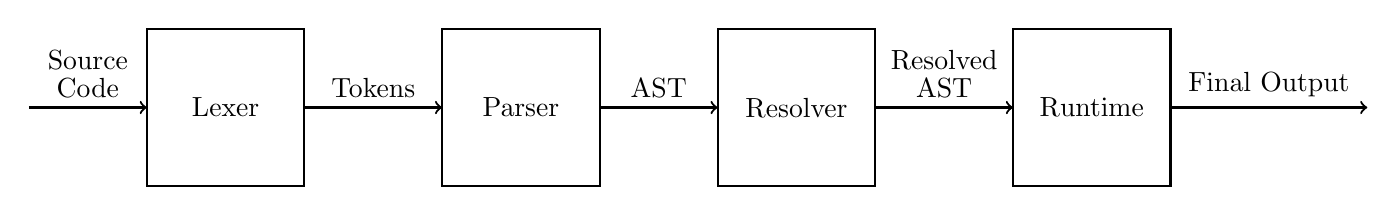
\begin{tikzpicture}
    % Draw the boxes
    \draw[thick] (-4.5, 0) rectangle (-2.5, 2);
    \draw[thick] (-0.75, 0) rectangle (1.25, 2);
    \draw[thick] (2.75, 0) rectangle (4.75, 2);
    \draw[thick] (6.50, 0) rectangle (8.50, 2);
    
    % Labels inside the boxes
    \node at (-3.5, 1) {Lexer};
    \node at (0.25, 1) {Parser};
    \node at (3.75, 1) {Resolver};
    \node at (7.5, 1) {Runtime};
    
    % Arrows and labels between boxes
    \draw[->, thick] (-2.5, 1) -- (-0.75, 1) node[midway, above] {Tokens};
    \draw[->, thick] (1.25, 1) -- (2.75, 1) node[midway, above] {AST};
    \draw[->, thick] (4.75, 1) -- (6.50, 1) node[midway, above] {\shortstack{Resolved \\ AST}};
    
    % Input and output arrows
    \draw[->, thick] (-6, 1) -- (-4.5, 1) node[midway, above] {\shortstack{Source \\ Code}};
    \draw[->, thick] (8.50, 1) -- (11, 1) node[midway, above] {Final Output};
  \end{tikzpicture}
  \caption{Box-Diagram representing the phases of the Bleach Interpreter.}
\end{figure}

\subsection{Lexer/Scanner}
When it comes to the lexer/scanner, it's worth remembering the reader that its goal is to transform the received source code (which is viewed by it as a large string of characters) into a sequence of tokens that will be fed to the parser of the interpreter. Such transformation performed by the lexer is known as lexical analysis.

When it comes to the possible tokens to be generated during the lexical analysis, these are the following types of tokens recognized by the lexer:

\begin{itemize}
    \item \textbf{Single-Character Tokens:}
    \begin{table}[h]
    \centering
        \begin{tabular}{|c|c|}
        \hline
        \textbf{Token Type} & \textbf{Token} \\ \hline
        LEFT\_PAREN & \texttt{(} \\ \hline
        RIGHT\_PAREN & \texttt{)} \\ \hline
        LEFT\_BRACKET & \texttt{[} \\ \hline
        RIGHT\_BRACKET & \texttt{]} \\ \hline
        LEFT\_BRACE & \texttt{\{} \\ \hline
        RIGHT\_BRACE & \texttt{\}} \\ \hline
        COMMA & \texttt{,} \\ \hline
        DOT & \texttt{.} \\ \hline
        COLON & \texttt{:} \\ \hline
        SEMICOLON & \texttt{;} \\ \hline
        QUESTION\_MARK & \texttt{?} \\ \hline
        PLUS & \texttt{+} \\ \hline
        MINUS & \texttt{-} \\ \hline
        STAR & \texttt{*} \\ \hline
        SLASH & \texttt{/} \\ \hline
        REMAINDER & \texttt{\%} \\ \hline
        BANG & \texttt{!} \\ \hline
        EQUAL & \texttt{=} \\ \hline
        GREATER & \texttt{>} \\ \hline
        LESS & \texttt{<} \\ \hline
        \end{tabular}
        \caption{Single-Character Tokens recognized by the Lexer of Bleach's Interpreter. \newline \newline \newline}
    \end{table}

    \item \textbf{Double-Character Tokens:}
    \begin{table}[H]
    \centering
        \begin{tabular}{|c|c|}
        \hline
        \textbf{Token Type} & \textbf{Token} \\ \hline
        ARROW & \texttt{->} \\ \hline
        EQUAL\_EQUAL & \texttt{==} \\ \hline
        EQUAL\_EQUAL & \texttt{!=} \\ \hline
        GREATER\_EQUAL & \texttt{>=} \\ \hline
        LESS\_EQUAL & \texttt{<=} \\ \hline        
        \end{tabular}
        \caption{Double-Character Tokens recognized by the Lexer of Bleach's Interpreter.}
    \end{table}

    \item \textbf{Multi-Character Tokens:}
    \begin{table}[H]
    \centering
        \begin{tabular}{|c|c|}
        \hline
        \textbf{Token Type} & \textbf{Token} \\ \hline
        IDENTIFIER & \texttt{(a-z|A-Z|\_)(a-z|A-Z|0-9|\_)\textsuperscript{*}} \\ \hline
        NUMBER & \texttt{[0-9]\textsuperscript{+}(.[0-9]\textsuperscript{+})?} \\ \hline
        STRING & \texttt{"(any ASCII character)\textsuperscript{*}"} \\ \hline      
        \end{tabular}
        \caption{Multi-Character Tokens recognized by the Lexer of Bleach's Interpreter.}
    \end{table}

    \item \textbf{FILE\_END Token:} This token is a special one that the Bleach interpreter supports. It is responsible for signaling the end of a \texttt{.bch} file. This token has an empty string as its lexeme. Its addition will be discussed on section 4.5.
\end{itemize}

When talking about tokens, specially identifier tokens, it is important to provide the table of keywords of a programming language. In Bleach's case, this table is shown below:
\begin{table}[H]
    \centering
    \begin{tabular}{|c|c|c|}
    \hline
    \texttt{and} & \texttt{break} & \texttt{class}  \\ \hline
    \texttt{continue} & \texttt{do} & \texttt{elif}  \\ \hline
    \texttt{else} & \texttt{false} & \texttt{for}  \\ \hline
    \texttt{function} & \texttt{if} & \texttt{inherits} \\ \hline
    \texttt{lambda} & \texttt{let} & \texttt{method} \\ \hline
    \texttt{nil} & \texttt{or} & \texttt{print} \\ \hline
    \texttt{return} & \texttt{self} & \texttt{super} \\ \hline
    \texttt{true} & \texttt{while} &  \\ \hline
    \end{tabular}
    \caption{Table with all keywords available in Bleach.}
\end{table}

Regarding the implementation of the lexer itself, the road taken to achieve such goal was to build a hand-written lexer.

The implemented hand-written lexer can successfully recognize string literals and number literals. It can also ignore whitespace characters, single-line comments and multi-line comments. On top of that, the lexer is able to successfully distinguish token that share the same initial characters on their lexemes by using the concept of lookahead and "maximal munch", both previously presented. The "maximal munch" concept is also used to identify tokens that have a keyword as their lexemes from tokens that have just an identifier as their lexemes. 

Lastly, the lexer is capable of identifying invalid characters, unterminated string literals, unterminated multi-line comments and misuse of the \texttt{':'} character.

\subsection{Parser}
When it comes to the parser, it's worth remembering the reader that its goal is to transform the received sequence of tokens into an Abstract Syntax Tree (AST) that will be fed to the resolver of the interpreter. This conversion executed by the parser is known as syntax analysis.

Regarding the possible AST nodes to be generated during the syntax analysis, they can be divided into two groups of nodes (expressions and statements). These groups are structured as displayed below:

\begin{table}[h!]
\centering
    \begin{tabular}{|c|c|}
    \hline
    \textbf{Expr} & \textbf{Stmt} \\ \hline
    Assign & Block \\ \hline
    Binary & Break \\ \hline
    Call & Class \\ \hline
    Get & Continue \\ \hline
    Grouping & DoWhile \\ \hline
    LambdaFunction & Expression \\ \hline
    ListLiteral & For \\ \hline
    Literal & Function \\ \hline
    Logical & If \\ \hline
    Self & Print \\ \hline
    Set & Return \\ \hline
    Super & Var \\ \hline  
    Ternary & While \\ \hline
    Unary &  \\ \hline
    Variable &  \\ \hline
    \end{tabular}
    \caption{All possible types of AST nodes in the Bleach programming language. \newline}
\end{table}

With respect to the parsing technique that is behind the parser component of the implemented Bleach interpreter, the chosen one was the Recursive-Descent parsing technique.


\subsection{Resolver}



\subsection{Interpreter/Runtime}

\section{Challenges, Decisions and Trade-Offs}
\textbf{Em Lexer: Falar sobre a decisão de escolher um hand-written lexer, comparar com outras opções. Desafios para lidar com o reconhecimento de strings, identificadores, numeros, comentários, "maximal munch" theorem, e suporte à funções nativas (uso de ':').}

\textbf{Falar sobre implementação de funções nativas: permissão do uso do caracter ':' em certos casos (restritos pelo Lexer.hpp e pelo Parser.hpp). Falar sobre a implementação das funções nativas em si dentro do arquivo "NativeFunctions.hpp'. Falar sobre o binding feito em escopo global do interpretador para permitir o acesso às funções nativas e no método VisitCallExpr do arquivo 'Interpreter.hpp'.}

\textbf{Em Parser: Falar sobre a decisão de escolher um hand-written parser que segue a abordagem top-down recursive.}

\textbf{Falar sobre a decisão de permitir a redeclaração de variáveis globais em Bleach e o porquê disso.}

\textbf{Falar sobre a decisão de implementar single-inheritance ao invés de multiple-inheritance. Isso pode entrar tanto como "Future Work" como ser um assignment para uma turma.}

\textbf{Falar sobre a decisão de usar um Handwritten Lexer/Scanner.}

\textbf{Falar sobre a decisão de usar Recursive-Descent Parsing.}

\textbf{Falar sobre a decisão de usar um Tree-Walk Interpreter ao invés de uma ByteCode VM ou de um Compilador.}


\section{What Makes Bleach Shine and How It Can Be Used In a Classroom Environment}
\chapter{Evaluation} \label{cap:Resultados}

\begin{displayquote}
    \begin{center}
        \textit{``There is no pain as long as I keep my eyes on the balance scale.''}
    \end{center}
\end{displayquote}

\begin{flushright}
   \textit{-- NORIAKI KUBO}
\end{flushright}

% \section{Introduction}
This chapter is dedicated to present to the reader a series of different approaches that were taken in order to test the Bleach programming language and the Tree-Walk Interpreter implemented for it from different perspectives. Regarding these perspectives, the following approaches were taken:
\begin{itemize}
    \item \textbf{Test Suite:} A Test Suite is a carefully tailored collection of test cases and test scripts implemented in order to verify that a software program or a specific module of a program is behaving as expected.
    
    \item \textbf{Implementation of famous Algorithms and Data Structures:} As a way to better demonstrate Bleach's expressiveness and prowess, this section is dedicated to present to the reader implementation of famous Algorithms and Data Structures commonly taught in an undergraduate Computer Science degree.
    
    \item \textbf{Comparison of Bleach with ChocoPy, Cool and MiniJava:} Regarding comparison with its predecessors, this section is dedicated to compare Bleach with them in terms of language features.
\end{itemize}


\section{Bleach's Test Suite}
As mentioned above, one of the different ways to evaluate Bleach was through the creation of a test suite that verifies the correctness of the Tree-Walk Interpreter implementation. In this particular scenario, this test suite is composed of several test cases, the expected output for each of these test cases and a test script responsible for executing the test cases automatically.

The Test Suite is made of 44 test cases and a shell script that executes these tests in an automated manner. These test cases are divided into 3 groups (tests responsible for Expression nodes, tests responsible for Statement nodes and tests responsible for some of the Bleach Native Functions). All types of AST nodes previously presented in Table~\ref{tab:ASTNodes} are covered. Moreover, from these 44 test cases there are 2 of them that cover native functions from the following namespaces: \texttt{std::math} and \texttt{std::utils}.

Each test case is composed by a Bleach file (\texttt{.bch} extension) representing the Bleach program that will be executed by the interpreter, a file with the extension 
 \texttt{.bch.expected}, representing the expected output for that corresponding \texttt{.bch} file when it is executed and, finally, a corresponding \texttt{.bch.log} file that represents the actual output generated by the execution of such \texttt{.bch} file. In this context, it is important to highlight that each Bleach file (\texttt{.bch} extension) and its corresponding expected output (\texttt{.bch.expected} extension) were hand-crafted adopting an approach very similar to unit tests. Therefore, the focus of each test is on the runtime behavior of a single type of AST node. Finally, the difference between the \texttt{.bch.expected} and the \texttt{.bch.log} is computed. If there are no differences, then it means that the particular test case passed. Otherwise, it did not.

 This process is automated by a shell script called \texttt{bleach\_test\_pipeline.sh} that automatically executes each Bleach program and compares its expected output file with the produced output file. In the end, this script provides a simple metric displaying how many of the test cases have passed from the total number and it also shows which test cases did not pass.

 More detailed information about how to execute Bleach's test suite can be found at Bleach's official GitHub repository \cite{bleach_lang_git_repo}.


\section{Implementing Famous Algorithms and Data Structures in Bleach}
The main goal here is show the expressiveness and prowess of Bleach by demonstrating that it is possible to implement famous algorithms and data structures that are usually taught in an undergraduate "Introduction to Algorithms" course. These implementations, along with a few tests cases, can be found at \href{https://github.com/vmmc2/Bleach/tree/main/tests/algorithms_and_data_structures}{Famous A \& DS implementations in Bleach}. The implemented algorithms and data structures were:
\begin{itemize}
    \item Binary Heap
    \item Binary Search Tree
    \item Binary Search
    \item Breadth First Search
    \item Depth First Search
    \item Dijkstra's Shortest-Path Algorithm
    \item Insertion Sort
    \item Merge Sort
    \item Queue
    \item Quick Sort
    \item Stack
\end{itemize}

\begin{comment}

\begin{itemize}
    \item Stack
        \begin{lstlisting}
class Node{
  method init(value){
    self.value = value;
    self.next = nil;
  }

  method str(){
    return self.value;
  }
}

class Stack{
  method init(){
    self.root = nil;
    self.length = 0;
  }

  method empty(){
    return self.length == 0 ? true : false;
  }

  method size(){
    return self.length;
  }

  method push(value){
    let newNode = Node(value);
    if(self.root == nil){
      self.root = newNode;
    }else{
      newNode.next = self.root;
      self.root = newNode;
    }

    self.length = self.length + 1;

    return nil;
  }

  method pop(){
    if(self.root == nil){
      return "The stack is empty.";
    }else{
      let poppedValue = self.root;
      self.root = self.root.next;

      self.length = self.length - 1;

      return poppedValue;
    }
  }

  method str(){
    let stackAsString = "";
    let curr = self.root;
    while(curr != nil){
      stackAsString = stackAsString + (curr.value + " -> ");
      curr = curr.next;
    }
    stackAsString = stackAsString + " nil";

    return stackAsString;
  }

  method top(){
    if(self.root == nil){
      return "The stack is empty.";
    }else{
      return self.root;
    }
  }
}
        \end{lstlisting}


    \item Queue
        \begin{lstlisting}
class Node{
  method init(value){
    self.value = value;
    self.next = nil;
  }

  method str(){
    return self.value;
  }
}

class Queue{
  method init(){
    self.left = nil;
    self.right = nil;
    self.length = 0;
  }

  method empty(){
    return self.length == 0 ? true : false;
  }

  method size(){
    return self.length;
  }

  method front(){
    if(self.left == nil){
      return "The queue is empty.";
    }else{
      return self.left;
    }
  }

  method back(){
    if(self.right == nil){
      return "The queue is empty.";
    }else{
      return self.right;
    }
  }

  method push(value){
    if(self.length == 0){
      let newNode = Node(value);
      self.left = newNode;
      self.right = self.left;
    }else{
      let newNode = Node(value);
      self.right.next = newNode;
      self.right = newNode;
    }

    self.length = self.length + 1;

    return;
  }

  method pop(){
    if(self.length == 0){ // Queue is empty.
      return "The queue is empty.";
    }elif(self.length == 1){ // Queue is not empty and has only one element.
      let poppedValue = self.left.value;

      self.left = nil;
      self.right = nil;

      self.length = self.length - 1;

      return poppedValue;
    }else{ // Queue is not empty and has more than one element.
      let poppedValue = self.left.value;

      self.left = self.left.next;
      self.length = self.length - 1;

      return poppedValue;
    }
  }

  method str(){
    let queueAsString = "front -> ";
    let curr = self.left;
    while(curr != nil){
      if(curr != nil and curr.next != nil){
        queueAsString = queueAsString + (curr.value + " -> ");
      }else{
        queueAsString = queueAsString + curr.value;
      }
      curr = curr.next;
    }
    queueAsString = queueAsString + " <- back";

    return queueAsString;
  }
}
        \end{lstlisting}


    \item Insertion Sort
        \begin{lstlisting}
/*
Code that implements the Insertion Sort algorithm.
Assumes it is a list where every value is of type 'num'.
*/

function insertionSort(l){
  let n = l.size();

  for(let i = 0; i < n; i = i + 1){
    let curr = i;
    while(curr > 0 and l.getAt(curr) < l.getAt(curr - 1)){
      let temp = l.getAt(curr);
      l.setAt(curr, l.getAt(curr - 1));
      l.setAt(curr - 1, temp);
      curr = curr - 1;
    }
  }

  return;
}
        \end{lstlisting}
    \item Merge Sort
        \begin{lstlisting}
/*
Code that implements the Merge Sort algorithm.
Assumes it is a list where every value is of type 'num'.
*/

function merge(a, b){
  let n = a.size();
  let m = b.size();

  let i = 0;
  let j = 0;
  let k = 0;
  
  let c = [];
  c.fill(nil, m + n);

  while(i < n or j < m){
    if(j == m or (i < n and a.getAt(i) < b.getAt(j))){
      c.setAt(k, a.getAt(i));
      k = k + 1;
      i = i + 1;  
    }else{
      c.setAt(k, b.getAt(j));
      k = k + 1;
      j = j + 1;
    }
  }

  return c;
}

function mergeSort(a){
  if(a.size() <= 1){
    return a;
  }else{
    let b = [];
    let c = [];
    let n = a.size();
    let mid = std::math::floor(n/2 - 1);

    for(let i = 0; i <= mid; i = i + 1){
      b.append(a.getAt(i));
    }

    for(let i = mid + 1; i <= n - 1; i = i + 1){
      c.append(a.getAt(i));
    }

    b = mergeSort(b);
    c = mergeSort(c);

    return merge(b, c);
  }
}
        \end{lstlisting}
    
    
    \item Quick Sort
        \begin{lstlisting}
/*
Code that implements the Quick Sort algorithm.
Assumes it is a list where every value is of type 'num'.
*/

function swap(list, a, b){
  let temp = list.getAt(a);
  list.setAt(a, list.getAt(b));
  list.setAt(b, temp);

  return;
}

function partition(list, low, high){
  let pivot = list.getAt(high);
  let i = low - 1;

  for(let j = low; j <= high - 1; j = j + 1){
    if(list.getAt(j) <= pivot){
      i = i + 1;
      swap(list, i, j);
    }
  }
  swap(list, i + 1, high);

  return i + 1;
}

function quickSort(list, low, high){
  if(low < high){
    let q = partition(list, low, high);
    quickSort(list, low, q - 1);
    quickSort(list, q + 1, high);
  }

  return;
}
        \end{lstlisting}
    
    
    
    \item Binary Search
        \begin{lstlisting}
function binarySearch(list, target){
  let left = 0;
  let right = list.size() - 1;

  while(left <= right){
    let mid = std::math::floor((left + right) / 2);
    if(list.getAt(mid) == target){
      return mid;
    }elif(list.getAt(mid) > target){
      right = mid - 1;
    }else{
      left = mid + 1;
    }
  }

  return -1; // Target value not present inside the list.
}
        \end{lstlisting}
    \item Binary Search Tree (BST)
        \begin{lstlisting}
/*
Code that implements the Binary Search Tree data-structure by using a pointers approach.
*/

class TreeNode{
  method init(key, value){
    self.key = key;
    self.value = value;
    self.left = nil;
    self.right = nil;
  }

  method str(){
    return "Node Key: " + self.key + " - Node Value: " + self.value;
  }
}

class BST{
  method init(){
    self.root = nil;
    self.length = 0;
  }

  method insert(key, value){
    if(self.root == nil){
      self.root = TreeNode(key, value);
    }else{
      let curr = self.root;
      while(true){
        if(key < curr.key and curr.left == nil){
          curr.left = TreeNode(key, value);
          break;
        }elif(key < curr.key and curr.left != nil){
          curr = curr.left;
        }elif(curr.key < key and curr.right == nil){
          curr.right = TreeNode(key, value);
          break;
        }else{
          curr = curr.right;
        }
      }
    }

    self.length = self.length + 1;

    return;
  }

  method aux_delete(root, key){
    if(root == nil){
      return root;
    }

    if(key < root.key){
      root.left = self.aux_delete(root.left, key);
    }elif(key > root.key){
      root.right = self.aux_delete(root.right, key);
    }else{
      // Scenario where the node to be deleted has one child or no child.
      if(root.left == nil){
        return root.right;
      }elif(root.right == nil){
        return root.left;
      }

      // Scenario where the node to be deleted has two children.
      // In this case, the inorder sucessor of the node to be deleted is retrieved:
      let temp = self.findMinimum(root.right);

      // Replacing the root's key and value with its inorder successor's key and value:
      root.key = temp.key;
      root.value = temp.value;

      // Deleting the inorder successor:
      root.right = self.aux_delete(root.right, temp.key);
    }

    return root;
  }

  method delete(key){
    self.root = self.aux_delete(self.root, key);
    self.length = self.length - 1;

    return;
  }

  method find(key){
    let curr = self.root;

    while(curr != nil and curr.key != key){
      if(key < curr.key){
        curr = curr.left;
      }else{
        curr = curr.right;
      }
    }

    return curr == nil ? "Could not find the key inside the BST" : curr;
  }

  method size(){
    return self.length;
  }

  method findMinimum(node){
    let curr = node;

    while(curr.left != nil){
      curr = curr.left;
    }

    return curr;
  }

  method inorderTraversal(curr){
    if(curr == nil){
      return;
    }
    self.inorderTraversal(curr.left);
    std::io::print(curr);
    self.inorderTraversal(curr.right);
  
    return;
  }
}
        \end{lstlisting}

    
    \item Binary Heap
        \begin{lstlisting}
/*
Code that implements the Binary Min Heap data-structure.
*/

class MinBinaryHeap{
  method init(){
    self.heap = [];
  }

  method empty(){
    return self.size() == 0 ? true : false;
  }

  method size(){
    return self.heap.size();
  }

  method top(){
    if(self.size() == 0){
      return "The Binary Heap is empty!";
    }else{
      return self.heap.getAt(0);
    }
  }

  method pop(){
    if(self.size() == 0){
      return "The Binary Heap is empty!";
    }else{
      self.swap(0, self.size() - 1);

      let minValue = self.heap.pop();
      self.bubbleDown(0);

      return minValue;
    }
  }

  method push(value){
    self.heap.append(value);
    self.bubbleUp(self.size() - 1);

    return;
  }

  method swap(i, j){
    let temp = self.heap.getAt(i);
    self.heap.setAt(i, self.heap.getAt(j));
    self.heap.setAt(j, temp);

    return;
  }

  method bubbleDown(index){
    let smallest = index;
    let leftChild = 2 * index + 1;
    let rightChild = 2 * index + 2;

    if(leftChild < self.heap.size() and self.heap.getAt(leftChild) < self.heap.getAt(smallest)){
      smallest = leftChild;
    }

    if(rightChild < self.heap.size() and self.heap.getAt(rightChild) < self.heap.getAt(smallest)){
      smallest = rightChild;
    }

    if(smallest != index){
      self.swap(index, smallest);
      self.bubbleDown(smallest);
    }

    return;
  }

  method bubbleUp(index){
    let parentIndex = std::math::floor((index - 1) / 2);
    if(index > 0 and self.heap.getAt(index) < self.heap.getAt(parentIndex)){
      self.swap(index, parentIndex);
      self.bubbleUp(parentIndex);
    }

    return;
  }
}
        \end{lstlisting}


    \item Depth First Search (DFS)
        \begin{lstlisting}
function dfs(source, adjacencyList, visitingOrder, visited){
  visited.setAt(source, true);
  visitingOrder.append(source);

  for(let i = 0; i < adjacencyList.getAt(source).size(); i = i + 1){
    let neighbor = adjacencyList.getAt(source).getAt(i);
    if(!visited.getAt(neighbor)){
      dfs(neighbor, adjacencyList, visitingOrder, visited);
    }
  }

  return;
}
        \end{lstlisting}

        
    \item Breadth First Search (BFS)
        \begin{lstlisting}
function bfs(source, adjacencyList, visited, distance){
  visited.setAt(source, true);
  distance.setAt(source, 0);

  let queue = Queue();
  queue.push(source);

  while(!queue.empty()){
    let currNode = queue.pop();

    for(let i = 0; i < adjacencyList.getAt(currNode).size(); i = i + 1){
      let neighbor = adjacencyList.getAt(currNode).getAt(i);

      if(!visited.getAt(neighbor)){
        visited.setAt(neighbor, true);
        distance.setAt(neighbor, 1 + distance.getAt(currNode));
        queue.push(neighbor);
      }
    }
  }

  return;
}
        \end{lstlisting}
    \item Dijkstra's Shortest Path Algorithm
        \begin{lstlisting}
function dijkstraAlgorithm(source, adjacencyList, distance){
  let minHeap = MinBinaryHeap(); // Modified to receive lists of 2 elements.
  distance.setAt(source, 0);

  minHeap.push([0, source]);

  while(!minHeap.empty()){
    let currNodeInfo = minHeap.pop();
    let minPath = currNodeInfo.getAt(0);
    let currNode = currNodeInfo.getAt(1);

    for(let i = 0; i < adjacencyList.getAt(currNode).size(); i = i + 1){
      let neighbour = adjacencyList.getAt(currNode).getAt(i).getAt(0);
      let edge = adjacencyList.getAt(currNode).getAt(i).getAt(1);
      if(distance.getAt(currNode) + edge < distance.getAt(neighbour)){
        distance.setAt(neighbour, distance.getAt(currNode) + edge);
        minHeap.push([distance.getAt(neighbour), neighbour]);
      }
    }
  }

  return;
}
        \end{lstlisting}
\end{itemize}

\newpage

\end{comment}

\newpage

\section{Comparing Bleach with ChocoPy, Cool and MiniJava}
In this section, a comparison between Bleach, ChocoPy, Cool and MiniJava is presented in Table 5.1 in terms of the features available in these programming languages.


\begin{table}[h!]
    \centering
    \begin{tabular}{|p{3.2cm}|p{3cm}|p{3cm}|p{3cm}|p{3cm}|p{3cm}|}
        \hline
        \textbf{Feature} & \textbf{Bleach} & \textbf{ChocoPy} & \textbf{Cool} & \textbf{MiniJava} \\  % First row: header
        \hline
        \textbf{Type System} & Dynamically-Typed & Statically-Typed & Statically-Typed & Statically-Typed \\  % Data rows
        \hline
        \textbf{Built-In Types} & \texttt{bool}, \texttt{nil}, \texttt{num}, \newline \texttt{list}, \texttt{str} & \texttt{int}, \texttt{bool}, \texttt{None}, \texttt{list}, \texttt{str} & \texttt{Int}, \texttt{Bool}, \texttt{String} & \texttt{int}, \texttt{int[ ]} \texttt{boolean}, \texttt{void} \\
        \hline
        \textbf{Arithmetical Operators} & \texttt{+}, \texttt{-}, \texttt{*}, \texttt{/}, \texttt{\%} & \texttt{+}, \texttt{-}, \texttt{*}, \texttt{//}, \texttt{\%} & \texttt{+}, \texttt{-}, \texttt{*}, \texttt{/} & \texttt{+}, \texttt{-}, \texttt{*} \\
        \hline
        \textbf{Comparison Operators} & \texttt{>}, \texttt{>=}, \texttt{<}, \texttt{<=} & \texttt{>}, \texttt{>=}, \texttt{<}, \texttt{<=} & \texttt{<}, \texttt{<=} & \texttt{<} \\
        \hline
        \textbf{Equality Operators} & \texttt{==}, \texttt{!=} & \texttt{==}, \texttt{!=}, \texttt{is} & \texttt{=} & No support \\
        \hline
        \textbf{Logical Operators} & \texttt{and}, \texttt{or}, \texttt{!} & \texttt{and}, \texttt{or}, \texttt{not} & \texttt{not} & \texttt{\&\&}, \texttt{!} \\
        \hline
        \textbf{Assignment Operator} & \texttt{=} & \texttt{=} & \texttt{<-} & \texttt{=} \\
        \hline
        \textbf{Ternary Operator Support} & Yes & Yes & No & No \\
        \hline
        \textbf{If Statement Support} & \texttt{if}, \texttt{elif}, \texttt{else} & \texttt{if}, \texttt{elif}, \texttt{else} & \texttt{if}, \texttt{else} & \texttt{if}, \texttt{else} \\
        \hline
        \textbf{Loops Support} & \texttt{for}, \texttt{do-while}, \texttt{while} & \texttt{while}, \texttt{for in} (only in lists and strings) & \texttt{while} & \texttt{while} \\
        \hline
        \textbf{Break/Continue Statements Support} & Yes, Yes & No, No & No, No & No, No \\
        \hline
        \textbf{Function Declaration Support} & Yes (with the \texttt{function} keyword) & Yes (with the \texttt{def} keyword) & Yes (only method declaration within classes) & Yes (only method declaration within classes) \\
        \hline
        \textbf{Anonymous Function Support} & Yes (with the \texttt{lambda} keyword) & No & No & No \\
        \hline
        \textbf{Comments} & Single-line (\texttt{//}) and Multi-line (\texttt{/**/}) & Single-Line (\texttt{\#}) & Single-line (\texttt{---}) and Multi-line (\texttt{**}) & Single-line (\texttt{//}) and Multi-line (\texttt{/**/}) \\
        \hline
        \textbf{Language Paradigm} & Object-Oriented and Interpreted & Object-Oriented and Compiled & Object-Oriented and Compiled & Object-Oriented and Compiled \\
        \hline
        \textbf{Inheritance} & Single & Single & Single & Single \\
        \hline
    \end{tabular}
    \caption{Comparison between Bleach, ChocoPy, Cool and MiniJava.}
    \label{tab:example5x5}
\end{table}
\chapter{Conclusion and Future Work} \label{cap:conclusao}

\begin{displayquote}
    \begin{center}
        \textit{``Even without a form, we will never stop walking.''}
    \end{center}
\end{displayquote}

\begin{flushright}
   \textit{-- TITE KUBO}
\end{flushright}

\section{Conclusion}

\section{Future Work}


\appendix

\backmatter

% Referencias Bibliográficas
%\nocite{*}
\bibliographystyle{ieeetr}
\bibliography{References/references}

\end{document}
